\documentclass[12pt]{report}
\usepackage{holtex}
\usepackage{array}
\usepackage{skcformat}
\usepackage{authblk}
\usepackage{float}
\usepackage{rotating}
\usepackage[T1]{fontenc}

%% ---------------------------------------------------
%% Use biblatex
%% ---------------------------------------------------
% \usepackage[backend=biber,style=numeric]{biblatex}
% \addbibresource{Book.bib,references.bib,chapter6_references.bib}

% \usepackage[hyphens]{url}
%\usepackage[numbers, sort&compress]{natbib}
\usepackage[numbers]{natbib}
\usepackage{xurl}

%% -------------------------------------
%% hyperref without parameters outlines urls in teal boxes in bibliography
%% -------------------------------------
\usepackage{hyperref}
% \usepackage[colorlinks=true, linkcolor=black, urlcolor=black, citecolor=black]{hyperref}

\usepackage{enumitem}
\usepackage{textcomp}
\usepackage{titlesec}

% Page layout (use what's in skcformat.sty)
% \usepackage[top=1.3in, bottom=1in, left=1in, right=1in, headheight=0.75in, headsep=0.25in]{geometry}

% Graphics
\usepackage{graphicx}
\usepackage{eso-pic}
\usepackage{tikz}
\usetikzlibrary{calc}
\graphicspath{{Figures/}}

% Colors - CTR uses teal/cyan instead of orange
\usepackage{xcolor}
\usepackage{colortbl}  % For table row colors
\definecolor{nsablue}{RGB}{0,51,102}
\definecolor{nsateal}{RGB}{0,188,212}  % Teal/cyan color for CTR
\definecolor{ctrdarkblue}{RGB}{25,58,75}  % Dark blue for cover sidebar

%% ---------------------------------------------------
%% Packages for colorboxes
%% ---------------------------------------------------
\usepackage{tcolorbox}

% Patch commands to use mainpages style on all pages
\usepackage{etoolbox}
\patchcmd{\tableofcontents}{\thispagestyle{plain}}{\thispagestyle{mainpages}}{}{}
\patchcmd{\listoftables}{\thispagestyle{plain}}{\thispagestyle{mainpages}}{}{}
\patchcmd{\listoffigures}{\thispagestyle{plain}}{\thispagestyle{mainpages}}{}{}
\patchcmd{\chapter}{\thispagestyle{plain}}{\thispagestyle{mainpages}}{}{}

% Section numbering
\setcounter{secnumdepth}{4}
\setcounter{tocdepth}{4}

% Headers and Footers
\usepackage{fancyhdr}
\pagestyle{fancy}
\fancyhf{}

% Define the header background for running pages (pages 2+)
\newcommand{\ctrheaderbackground}{%
    \begin{tikzpicture}[remember picture,overlay]
        % Header background
        \node[anchor=north west, inner sep=0pt] at (current page.north west) {%
            \includegraphics[width=\paperwidth,height=0.75in]{header-background.jpg}%
        };
        % Teal line below header (CTR uses teal not orange)
        \draw[line width=3pt, nsateal] ([yshift=-0.75in]current page.north west) -- ([yshift=-0.75in]current page.north east);
    \end{tikzpicture}%
}

% Cover page style (no header/footer on cover)
\fancypagestyle{coverpage}{%
    \fancyhf{}
    \renewcommand{\headrulewidth}{0pt}
    \renewcommand{\footrulewidth}{0pt}
}

% Main pages style (Pages 2+) - FIXED: Background is drawn first, then logo and text on top
\fancypagestyle{mainpages}{%
    \fancyhf{}
    \fancyhead[L]{%
        \ctrheaderbackground% Draw background first
        \begin{tikzpicture}[remember picture,overlay]
            % Position logo on top of background
            \node[anchor=north west, inner sep=0pt] at ([xshift=0.5in, yshift=-0.15in]current page.north west) {%
                \includegraphics[height=0.4in]{nsa-logo.png}%
            };
            % Position text on top of background
            \node[anchor=west, inner sep=0pt] at ([xshift=1.15in, yshift=-0.35in]current page.north west) {%
                \parbox{6in}{\color{white}\fontsize{13}
%                {16}\selectfont\textbf{NSA | Landscape of %Government, Academic, and Industry Efforts in Responsible,
%Secure, and Trustworthy AI}}%
                 {16}\selectfont\textbf{NSA | Analysis of Research in Reliable, Secure, and Trustworthy AI}}%
           };
        \end{tikzpicture}%
    }
    \fancyfoot[L]{\small U/OO/\#-24 | PP-24-\#\#\#\# | Month 2024 Ver. 1.0}
    \fancyfoot[R]{\small\thepage}
    \renewcommand{\headrulewidth}{0pt}
    \renewcommand{\footrulewidth}{0pt}
}

% REMOVED: Don't use AddToShipoutPictureBG since mainpages style now handles it
% This was causing the issue where Chapter 2 (page 1 in arabic numbering) didn't get background
% \AddToShipoutPictureBG{%
%     \ifnum\value{page}>1
%         \ctrheaderbackground
%     \fi
% }

% Use roman numerals for front matter
\pagenumbering{roman}

% Listings for code
\usepackage{listings}
\usepackage{textcomp}

% Math packages
\usepackage{amsmath,amssymb}

% Other packages
\usepackage{shadow}
\usepackage{xspace}
\usepackage{soul}

\newcommand{\hlc}[2][yellow]{{%
    \colorlet{foo}{#1}%
    \sethlcolor{foo}\hl{#2}}%
}

% Column types
\newcolumntype{L}[1]{>{\raggedright\let\newline\\\arraybackslash\hspace{0pt}}p{#1}}
\newcolumntype{C}[1]{>{\centering\let\newline\\\arraybackslash\hspace{0pt}}p{#1}}
\newcolumntype{R}[1]{>{\raggedleft\let\newline\\\arraybackslash\hspace{0pt}}p{#1}}

\usepackage{calc}
\usepackage{booktabs}

% HOL packages
\usepackage{holtexbasic}
\usepackage{holtex}

\begin{document}

\input{our-content-macros}

%% ---------------------------------------------------
%% Cover Page with Two-Column Layout
%% ---------------------------------------------------
\thispagestyle{coverpage}

% Create the two-column cover page
\begin{tikzpicture}[remember picture,overlay]
    % Left sidebar - dark blue gradient with dots
    \fill[ctrdarkblue] (current page.north west) rectangle ([xshift=2.5in]current page.south west);
    
    % Add dot pattern to sidebar
    \node[anchor=north west, inner sep=0pt, opacity=0.3] at (current page.north west) {%
        \includegraphics[width=2.5in,height=\paperheight]{header-background.jpg}%
    };
    
    % NSA Logo on left sidebar
    \node[anchor=north west, inner sep=0pt] at ([xshift=0.5in, yshift=-1.5in]current page.north west) {%
        \includegraphics[height=1.2in]{nsa-logo.png}%
    };
    
    % Right side content - centered text
    % Title header
    \node[anchor=north, inner sep=0pt] at ([xshift=4.75in, yshift=-2in]current page.north west) {%
        \parbox{4.5in}{\raggedleft\fontsize{18}{22}\selectfont\textbf{National Security Agency\\Cybersecurity Technical Report}}%
    };
    
    % Main title
    \node[anchor=center, inner sep=0pt] at ([xshift=5.75in, yshift=-5in]current page.north west) {%
        \parbox{4.5in}{\raggedleft\fontsize{24}%
%        {30}\selectfont\textbf{Landscape of Government,
%cademic, and Industry Efforts in Responsible,
%Secure, and Trustworthy AI}}%
{30}\selectfont\textbf{Analysis of Research in Reliable,
Secure, and Trustworthy AI}}%
    };
     
    % Bottom info
    \node[anchor=south east, inner sep=0pt] at ([xshift=-0.5in, yshift=1.5in]current page.south east) {%
        \parbox{3in}{\raggedleft
            \fontsize{12}{16}\selectfont
            December, 2025\\[0.2cm]
            U/OO/\#-24\\
            PP-24-\#\#\#\#\\
            Version 1.0
        }%
    };
\end{tikzpicture}

\clearpage

%% ---------------------------------------------------
%% Front Matter - use mainpages style
%% ---------------------------------------------------
\pagestyle{mainpages}

\section*{Notices and history}
\addcontentsline{toc}{chapter}{Notices and History}

\subsection*{Document change history}
\vspace{-0.25in}
% Table without caption (not included in List of Tables)
\begin{table}[H]
\centering
\begin{tabular}{|p{2in}|p{1in}|p{3in}|}
\hline
\rowcolor{black!80}
\textcolor{white}{\textbf{Date}} & \textcolor{white}{\textbf{Version}} & \textcolor{white}{\textbf{Description}} \\
\hline
December, 2025 & 1.0 & Initial publication \\
\hline
%& & \\
\hline
\end{tabular}
\end{table}

\vspace{0.3cm}

\subsection*{Disclaimer of warranties and endorsement}

The information and opinions contained in this document are provided ``as is'' and without any warranties or guarantees. Reference herein to any specific commercial products, process, or service by trade name, trademark, manufacturer, or otherwise, does not constitute or imply its endorsement, recommendation, or favoring by the United States Government, and this guidance shall not be used for advertising or product endorsement purposes.

\vspace{0.3cm}

\subsection*{Trademark recognition}
Not applicable.
%Technology is a registered trademark of company. ‚ñ™ Technology is a registered trademark of company.

\vspace{0.3cm}

\subsection*{\textit{Acknowledgements}}

%NSA acknowledges 

\vspace{0.3cm}

\subsection*{Publication information}

\textbf{Author(s)}
Jae C. Oh, Shiu-Kai Chin, Matt Clark, Garrett Katz, and William Young
%National Security Agency (NSA)\\
%Cybersecurity Directorate

\vspace{0.3cm}

\noindent\textbf{Contact information}

\noindent Jae C. Oh, David G. Edelstein Professor, 2-187
Center for Science and Technology, College of
Engineering and Computer Science, Syracuse
University, Syracuse, NY 13244 |
\href{mailto:jcoh@syr.edu}{jcoh@syr.edu}

\noindent\textbf{Cybersecurity Report Feedback:} \href{mailto:CybersecurityReports@nsa.gov}{CybersecurityReports@nsa.gov}

\noindent\textbf{General Cybersecurity Inquiries or Customer Requests:} \href{mailto:Cybersecurity_Requests@nsa.gov}{Cybersecurity\_Requests@nsa.gov}

\noindent\textbf{Defense Industrial Base Inquiries and Cybersecurity Services:} \href{mailto:DIB_Defense@cyber.nsa.gov}{DIB\_Defense@cyber.nsa.gov}

\noindent\textbf{Media Inquiries / Press Desk:} NSA Media Relations: 443-634-0721, \href{mailto:MediaRelations@nsa.gov}{MediaRelations@nsa.gov}

\clearpage

%% ---------------------------------------------------
%% Purpose Section (on its own page)
%% ---------------------------------------------------

\subsection*{Purpose}

This document was developed in furtherance of NSA's cybersecurity missions, including its responsibilities to identify and disseminate threats, and to develop and issue cybersecurity specifications and mitigations. This information may be shared broadly to reach all appropriate stakeholders.

\clearpage

%\section*{Executive summary}
%\addcontentsline{toc}{chapter}{Executive Summary}

% Add your executive summary content here or use \input
\chapter{Executive Summary} \label{cha:alt-executive-summary}

%\vspace{-0.3in}
% \fbox{%
%   \begin{minipage}{\dimexpr\linewidth-2\fboxsep-2\fboxrule\relax}
%     \textbf{Summary of Main Points Bottom Line Up Front (BLUF)}
%     \begin{itemize}
%       \item When we say \emph{trustworthy artificial intelligence} we mean \textbf{trustworthy systems with AI as a subsystem}
%       \item This definition is consistent with the following standards
%         \begin{itemize}
%           \item NIST SP 800-160v1r1, Engineering Secure Trustworthy Systems, \cite{NIST800-160}
%           \item ISO/IEC/IEEE 15288, Systems and software engineering, System life cycle processes, \cite{ISO15288}
%         \end{itemize}
%     \end{itemize}
%   \end{minipage}%
% }

\section{Introduction}
Artificial Intelligence (AI) systems are rapidly being integrated into defense and critical infrastructure, yet a fundamental question remains largely unaddressed: how do we systematically ensure these systems are trustworthy for mission-critical operations? As AI capabilities advance and deployment accelerates, the need for rigorous, evidence-based approaches to AI trustworthiness becomes increasingly urgent. This report presents a comprehensive investigation of  54,628  AI research papers published between 2021 and 2025, mapped against established systems engineering frameworks and organizational risk management standards. Our analysis reveals a troubling disconnect between the technical focus of current AI research and the foundational requirements for mission assurance a gap that poses significant risks to national security and operational effectiveness.

%vspace{-1.5em}
\section{Our Findings}

Only 9,183 AI papers out of 54,628 AI papers examined dealt with any aspect of AI trustworthiness, reliability, or security. Virtually all AI papers related to trustworthiness, reliability, or security were at the lowest level of abstraction, namely the \emph{systems and operations} level. The vast majority of these papers dealt with AI models, AI implementations, and performance of AI algorithms and code. Few or none addressed problem requirements or provided evidence of trustworthiness. Few or none addressed larger concerns at the mission or business process level or at the organization and governance structure level.

\begin{figure}[h]
    \centering
    \includegraphics[width=1.0\linewidth]{STORM-AI Deliverable-1/Figures/Paper-Classification-Results.jpg}
    \caption{\it Results of searching and classifying 54,628 AI papers: fewer than 16.8\% address AI Trustworthiness, Reliability, or Security; few or none of those address organizational or mission requirements. \textbf{Mission Assurance is completely neglected.}}
    \label{fig:heatmapAlt}
\end{figure}

\section{Mission Assurance is Completely Neglected}

\textbf{Mission Assurance} \cite{DoD3020-40-MA} \emph{is a process to protect or ensure the continued function and resilience of capabilities and assets, including personnel, equipment, facilities, networks, information and information systems, infrastructure, and supply chains, critical to the execution of DoD mission-essential functions in any operating environment or condition}\footnote{Definition of Mission Assurance in DoD Directive 3020.40 Mission Assurance, September 2018}, where \textbf{Mission-Essential Functions} \cite{DoD3020-26-Continuity-MEF} \emph{are select functions directly related to accomplishing the Department's mission. Failure to perform or sustain these functions, which directly support PMEF, would significantly affect the Department of Defense's ability to provide vital services or exercise authority, direction, and
control}\footnote{Definition of Mission Essential Functions in DoD Directive 3020.26 DoD Continuity Policy, February 2018}. 

Our findings, illustrated in Figure~\ref{fig:heatmapAlt} show that existing AI research is disconnected from organization and mission requirements, and trustworthiness, with no systematic processes for guaranteeing mission essential functions in systems using AI. Developing  \textbf{mission-assurance processes for systems using AI must be a top priority}.

% -- Comments below are at the very end of component files --
% -- pointing to the main file --
% ---- this points LaTeX to STORM-AI-Deliverable-1.tex ---- 
% Local Variables: 
% TeX-master: "STORM-AI-Deliverable-1"
% End:

\section{Recommendations}

Addressing the documented gap in early-lifecycle mission context and requirements requires a disciplined, systems-level approach. Therefore, we recommend using the System-Theoretic and Technical Operational Risk Management (STORM) methodology \cite{STORM}, with particular emphasis on its STPA-SEC component \cite{STPA-SEC}. STPA-SEC is specifically designed to perform the essential tasks that are currently missing: generating mission objectives, identifying unacceptable losses and hazards, and defining the constraints that must govern system behavior. In doing so, it aligns policy intent with technical implementation and frames security as a mission-focused issue rather than just a technical challenge.
%\noindent\fbox{\parbox{\dimexpr\textwidth-2\fboxsep-2\fboxrule}{%
%\begin{center}
%\textbf{There is a clear opportunity to strengthen mission context, %early requirements definition, and downstream verification and %validation in AI trustworthiness research.}
%\end{center}
%}}
%\newline
\begin{tcolorbox}
 \textbf{There is a clear opportunity to strengthen mission context, early requirements definition, and downstream verification and validation in AI trustworthiness research.} 
\end{tcolorbox}

Once these mission requirements and constraints are established, STORM's Certified Security by Design (CSBD) component \cite{CSBD-IOT} \cite{CSBD-Education} enables formal verification that the system design satisfies them. CSBD provides evidence---not assumptions---that the implemented Concepts of Operation (CONOPS) enforce complete mediation, ensuring actions occur only if they are authorized and authenticated under the defined policy. This closes the loop between mission intent, system design, and verification, and delivers the kind of demonstrable trustworthiness and mission assurance required by NIST SP 800-160v1r1 \cite{nist_sp800_160v1}.

\clearpage

%% ---------------------------------------------------
%% Table of Contents
%% ---------------------------------------------------

\tableofcontents
\clearpage

\listoftables
\clearpage

\listoffigures
\clearpage

%% ---------------------------------------------------
%% Main Content - switch to arabic numbering
%% ---------------------------------------------------
\pagenumbering{arabic}

%\chapter{Introduction}
%\label{ch:introduction}
\chapter{Organization of the Report and Overview of Methodology}
% \label{chap:description}
% \fbox{%
%   \begin{minipage}{\dimexpr\linewidth-2\fboxsep-2\fboxrule\relax}
%     \textbf{Summary of Main Points Bottom Line Up Front (BLUF)}
%     \begin{itemize}
%       \item
%     \end{itemize}
%   \end{minipage}%
% }

\section{Introduction}

This chapter outlines the structure of this report and describes our approach to surveying and classifying research articles, reports, and standards related to AI trustworthiness. Understanding how current research and industry efforts are organized across organizational tiers and systems engineering lifecycle phases is essential for identifying gaps and directing future efforts toward mission-secure, trustworthy AI systems for defense applications.

A key challenge in AI trustworthiness research is the lack of agreement within the community on what defines ''trust'' and ''trustworthiness.'' Different organizations, researchers, and practitioners use these terms inconsistently, leading to fragmented approaches and making it difficult to compare or combine different efforts. Some see trust as a technical property of systems, while others view it as a subjective judgment by stakeholders. This definitional ambiguity hampers the field's ability to make systematic progress.


To address this lack of agreement, we base our work on established standards and frameworks. For this deliverable, we categorize articles, reports, and standards using ISO/IEC/IEEE 15288~\cite{ISO15288} (systems and software engineering lifecycle processes) and NIST SP 800-39~\cite{nist_sp800_39} (risk management strategy for organizational tiers). We also consider NIST SP 800-160v1~\cite{nist_sp800_160v1} (systems security engineering), SP 800-37~\cite{nist_sp800_37} (risk management framework), and the AI Risk Management Framework (AI RMF 1.0)~\cite{nist_ai_rmf_2023} to develop best practices. By aligning our analysis with these standards, we ensure that our work has a consistent, authoritative basis that others in the defense and AI security communities can reference and build upon.

\section{Report Organization}

This report is organized to provide a comprehensive analysis of the current state of AI trustworthiness research and practice, culminating in our proposed STORM-AI framework. Each chapter has a specific role in helping us understand, design, and develop trustworthy, mission-secure systems for defense applications.\\

%\subsection{Road map of the Document Onward}

\noindent\textbf{Chapter 2: Organization of the Report and Methodology} (this chapter describes the overall structure of the report and our approach to the survey of articles, reports, and standards. It outlines the two-dimensional categorization framework using NIST SP 800-39 organizational tiers \cite{nist_sp800_39} and ISO/IEC/IEEE 15288  lifecycle phases \cite{ISO15288}.\\

\noindent\textbf{Chapter 3: Methodology for Survey of Articles and Reports and Their Categorization} provides comprehensive documentation of our systematic approach to collecting, categorizing, and validating the articles and reports. This chapter integrates three critical components:

\begin{itemize}[noitemsep]
    \item \textbf{Article and Report Sources and Collection} — Documents the government, academic, and industry sources surveyed, along with our automated collection methodology for processing 9,000+ papers efficiently
    
    \item \textbf{Two-Dimensional Categorization Framework} — Presents the detailed rubric based on NIST SP 800-39 organizational tiers and NIST SP 800-160/ISO 15288 lifecycle phases, including the complete set of questions used to categorize each document
    
    \item \textbf{LLM-Assisted Analysis with Human Validation} — Describes our three-stage hybrid approach that combines keyword filtering, multi-LLM categorization, and human validation to ensure reliability while enabling large-scale analysis
\end{itemize}

This chapter outlines our approach to ensuring reliability by following established meta-analysis best practices, including keyword-based inclusion criteria and inter-rater reliability measures such as percent agreement, Krippendorff's $\alpha$ \cite{hayes_krippendorff}, and Gwet's AC1 \cite{gwet_irr}. It reviews existing work on ensuring reliable outputs from LLMs and conducting systematic reviews of articles and reports, including PRISMA guidelines \cite{prisma2020} and recent studies on using LLMs for abstract screening. This methodological rigor is crucial for establishing the credibility of our findings and allowing other researchers to replicate our work. Code and data to reproduce our results are available in a private repository.
\footnote{For access, contact \texttt{gkatz01@syr.edu}.  The repository URL (only accessible after approval) is 
\url{https://drive.google.com/drive/folders/1wD__MxpJl9w_BoUalxbpZFoPehgvgHZh?usp=sharing}.}\\


\noindent\textbf{Chapter 4: Categorization Results} presents the visual representation of how existing work maps to our two-dimensional framework. These visualizations immediately reveal where research is concentrated and where critical gaps exist across organizational tiers and lifecycle phases.\\

\noindent\textbf{Chapter 5: Gaps and Recommendations} synthesizes the survey results to clearly identify deficiencies in current approaches. This chapter shows that while many organizations concentrate on tools and techniques during the implementation phase, the essential systems engineering work needed for mission-secure systems—especially in early lifecycle phases such as business and mission analysis, stakeholder needs definition, and system requirements definition—remains critically underdeveloped. The recommendations offer practical guidance for funding agencies, research institutions, and defense organizations.

\section{Scope and Methodology of Survey of Articles and Reports}

Our survey of articles and reports encompasses three primary domains: government publications and standards, academic research, and private industry efforts. We focused on work published between 2021 and 2025, capturing the recent surge in AI trustworthiness research while ensuring relevance to current technological capabilities and operational contexts.

Government sources include publications from NIST~\cite{nist_sp800_39,nist_sp800_160v1,nist_sp800_37,nist_ai_rmf_2023}, DoD~\cite{dod_ai_ethics}, DARPA~\cite{darpa_assured_autonomy}, and other defense and standards organizations. Publications by academic and industry research labs span peer-reviewed journals and conference proceedings in AI, security, systems engineering, and related fields. %Industry sources include white papers, technical reports, and frameworks from major technology companies and defense contractors.
We developed Python scripts to automate the download and extraction of abstracts from these sources, enabling efficient processing of large-scale academic articles and reports while maintaining data quality and consistency. The complete list of venues is presented in Chapter 3.

\subsection{Automated Abstract Collection}

Our automated collection pipeline performs the following operations:

\begin{enumerate}[noitemsep]
  \item \textbf{Paper Identification} --- Systematically crawls conference proceedings and journal archives to identify relevant papers published between 2021 and 2025
  
  \item \textbf{Metadata Extraction} --- Extracts title, authors, publication venue, year, and DOI/URL for each paper
  
  \item \textbf{Abstract Download} --- Retrieves abstracts through official APIs and reference export functions (where available) or structured web scraping %while respecting robots.txt protocols
  
  \item \textbf{Data Filtering and Validation} --- Verifies completeness of extracted data, filters based on trust-related keywords, and flags papers requiring manual review
  
  \item \textbf{Standardization} --- Formats all abstracts into a consistent structure for subsequent categorization
\end{enumerate}

This automated approach enabled us to process  54,628 papers (before keyword filtering) efficiently and consistently, maintain reproducibility by documenting all data sources and collection methods, reduce human error, support periodic updates, and focus human effort on the more cognitively demanding tasks of categorization and analysis.

\noindent\textbf{Government and Industry Sources.} We manually collected and processed government publications from NIST~\cite{nist_sp800_39,nist_sp800_160v1,nist_ai_rmf_2023}, DoD~\cite{dod_ai_ethics}, and DARPA~\cite{darpa_assured_autonomy}. These sources typically do not provide abstracts in a format amenable to automated collection. Industrial research labs of leading technology companies regularly publish at top conferences and are well-represented in our automatically-collected abstract dataset. For example, the seminal paper on transformers was co-authored by several Google research scientists and published at NeurIPS \cite{vaswani2017attention}.

\subsection{Two-Dimensional Categorization Framework} \label{sec:2D-X-Y}

All collected paper abstracts are categorized according to our two-dimensional framework. The X-axis represents 11 Systems Engineering Lifecycle Phases from ISO/IEC/IEEE 15288~\cite{ISO15288}. This lifecycle view is critical because trustworthiness properties must be established early and maintained throughout development. For mission-secure defense systems, deficiencies in early phases (particularly mission analysis and requirements definition) cannot be adequately compensated for in later phases.

The Y-axis represents the three Organizational Tiers defined in NIST SP 800-39~\cite{nist_sp800_39}. This tiered structure is essential for defense applications because trustworthiness must be maintained at all levels---from strategic organizational policies down to individual system implementations. Gaps at any tier can undermine mission security.

Each paper is assigned to one cell in this organizational tier $\times$ lifecycle phase matrix, enabling us to map the complete landscape of AI trustworthiness research and identify critical gaps in coverage.

\subsection{Importance of the Matrix View}

Understanding the complete landscape of AI trustworthiness research and practice is essential for:

\begin{itemize}[noitemsep]
\item\textbf{Identifying Critical Gaps.} By mapping all contributions across our two-dimensional framework, we can immediately identify where the community has concentrated its efforts and where significant gaps remain. For defense applications, understanding these gaps is crucial for risk management~\cite{nist_sp800_39,iso31000} and resource allocation.

\item\textbf{Avoiding Redundant Efforts.} A comprehensive landscape view prevents researchers from duplicating existing work, allowing them to focus on genuinely underserved areas. In resource-constrained defense environments, this efficiency is particularly valuable.

\item\textbf{Enabling Systematic Progress.} Rather than pursuing isolated improvements, the landscape view enables the community to systematically address the entire problem space. This is essential for achieving truly trustworthy systems, as vulnerabilities or gaps in any lifecycle phase or organizational tier can compromise overall mission security~\cite{nist_sp800_160v1,amodei2016concrete}.

\item\textbf{Guiding Future Research Priorities.} By revealing where foundational work is lacking, our analysis helps funding agencies, research institutions, and defense organizations prioritize investments in areas that will have the greatest impact on achieving trustworthy mission-secure AI systems~\cite{nist_ai_rmf_2023,ai_alignment}.

\item\textbf{Facilitating Integration and Interoperability.} Understanding how different efforts relate across tiers and lifecycle phases enables better integration of tools, methods, and frameworks. For complex defense systems involving multiple organizations and contractors, this integration capability is essential~\cite{nist_sp800_37,ISO15288}.
\end{itemize}

\section{Summary}

This chapter has outlined our systematic approach to surveying and categorizing articles and reports on AI trustworthiness, reliability, and security. Our two-dimensional framework---spanning organizational tiers and systems engineering lifecycle phases---provides the analytical structure necessary to identify where current efforts fall short of what is needed for mission-secure defense systems. The following chapters present our methodological rigor in using LLMs for analysis~\cite{li_llm_screening,dai_llm_literature}, survey results, and ultimately reveal critical gaps in current AI trustworthiness research and practice.

% -- Comments below are at the very end of component files
% -- pointing to the main file
% ---- this points LaTeX to STORM-AI-Deliverable-1.tex ---- 
% Local Variables: 
% TeX-master: "STORM-AI-Deliverable-1"
% End:

%\section{Audience}
% Add audience section content here

%\chapter{Mitigations}
%\label{ch:mitigations}
\chapter{Methodology for Surveying and Categorizing Articles and Reports}
\label{cha:methodology}

% This LaTeX file requires the enumitem package for [nosep] option
% Add to your preamble: \usepackage{enumitem}
% Add to your preamble: \usepackage{cite} or \usepackage{natbib}
% Include bibliography: \bibliography{chapter6_references}

\section{Overview and Motivation}

We use Large Language Models (LLMs) for our survey and meta-analysis of AI trustworthiness research articles and reports. Although LLMs offer tremendous potential to accelerate review processes---enabling the analysis of thousands of documents that would be impractical to review manually---they also introduce risks that must be carefully managed.



\subsection{Quality Assurance Approach}

To ensure the reliability of our LLM-assisted analysis, we implement multiple layers of verification. First, we write traditional scripts (without LLMs) to download all 54K abstracts from pre-determined, well-established publication venues.  This ensures that all surveyed papers are real, high quality, and accompanied by official working web links.  Next, we use traditional keyword-based filtering (without LLMs) to identify a subset of 9K abstracts relevant to trustworthy and secure systems with AI.  Finally, we use multiple LLMs and feed each of the 9K abstracts to each LLM, with the same detailed and carefully crafted prompt, using independent API calls for each abstract.  Furthermore, we validate LLM outputs against manual human categorization on a uniform random sample of 50 abstracts. This multi-layered approach ensures that any systematic errors or hallucinations will be quantified and corrected before they compromise the project's integrity.

\subsection{Objectives of This Chapter}

This chapter serves multiple complementary purposes:

\begin{enumerate}
\item \textbf{Methodological Transparency}: Document our approach so that others can evaluate and replicate our methods
\item \textbf{Risk Mitigation}: Identify potential failure modes and our strategies to prevent them
\item \textbf{Quality Assurance}: Establish validation procedures to detect and correct errors
\item \textbf{Best Practice Alignment}: Demonstrate that our approach follows established standards from both computer science and meta-analysis articles and practices
\item \textbf{Stakeholder Confidence}: Provide evidence that our LLM-assisted analysis is rigorous and reliable
\end{enumerate}

\subsection{Scope and Applicability}

While this chapter focuses on our specific application---surveying AI trustworthiness articles and reports---the principles and practices described are broadly applicable to systematic reviews of articles and reports in any technical domain, meta-analyses requiring categorization of large document sets, research synthesis projects where manual review is impractical, and any application of LLMs requiring high reliability and verifiability.

\section{Sources and Collection of Articles and Reports}

Our survey of articles and reports encompasses three primary domains: government publications and standards, academic research, and private industry efforts. We focused on work published between 2021 and 2025, capturing the recent five years of surge in AI trustworthiness research while ensuring relevance to current technological capabilities and operational contexts.

% \subsection{Government Sources}

% Government sources include publications from:
% \begin{itemize}
%     \item National Institute of Standards and Technology (NIST) -- including SP 800-39, SP 800-160 Vol. 1 Rev. 1, SP 800-37 Rev. 2, and AI Risk Management Framework (AI RMF 1.0)
%     \item Department of Defense (DoD) -- AI ethics principles and policy documents
%     \item Defense Advanced Research Projects Agency (DARPA)  program descriptions and technical reports
%     \item Other defense and standards organizations
% \end{itemize}

% \subsection{Academic Sources}

\subsection{Publication Sources}

To ensure comprehensive coverage of AI trustworthiness research across academia, industry, and government, we systematically collected articles and reports from multiple high-quality sources. Our academic articles and reports collection encompasses the following premier venues in artificial intelligence, machine learning, and related fields:

\begin{itemize}
    \item \textbf{AI and Society Journal} --\url{https://link.springer.com/journal/146}
    \begin{itemize}
        \item Springer journal focusing on societal implications of AI development and deployment
    \end{itemize}
    
    \item \textbf{AAAI/ACM Conference on AI, Ethics, and Society (AIES)} -- \url{https://www.aies-conference.com/2025/}
    \begin{itemize}
        \item Premier conference on responsible AI, fairness, and societal impacts
    \end{itemize}
    
    \item \textbf{ACM International Conference on Hybrid Systems: Computation and Control (HSCC)} --\url{https://hscc.acm.org/2025/}
    \begin{itemize}
        \item Conference on safety-critical cyber-physical systems and formal methods
    \end{itemize}
    
    \item \textbf{Annual AAAI Conference on Artificial Intelligence} --\url{https://aaai.org/conference/aaai/}
    \begin{itemize}
        %\item Association for the Advancement of Artificial Intelligence publications, including AI Magazine
        \item Top conference covering a broad spectrum of AI research including trustworthiness and security
    \end{itemize}
    
    \item \textbf{ACM SIGKDD} --\url{https://kdd.org/conferences}
    \begin{itemize}
        \item Knowledge Discovery and Data Mining conference proceedings
        \item Addresses privacy, fairness, and robustness in machine learning
    \end{itemize}
    
    \item \textbf{International Conference on Machine Learning (ICML)} -- \url{https://icml.cc/}
    \begin{itemize}
        \item Leading venue for machine learning research including robustness and safety
    \end{itemize}
    
    \item \textbf{Conference on Neural Information Processing Systems (NeurIPS)} -- \url{https://neurips.cc/}
    \begin{itemize}
        \item Premier conference featuring work on AI safety, alignment, and robustness
    \end{itemize}
    
    \item \textbf{North American Chapter of the Association for Computational Linguistics (NAACL)} -- \url{https://naacl.org/}
    \begin{itemize}
        \item Natural language processing research including bias and fairness in language models
    \end{itemize}
    
    \item \textbf{IEEE/CVF Computer Vision Conferences} -- \url{https://cvpr.thecvf.com/}
    \begin{itemize}
        \item Computer vision research including adversarial robustness and fairness
    \end{itemize}
    
    \item \textbf{International Conference on Autonomous Agents and Multiagent Systems (AAMAS)} --\url{https://aamas2025.org/} or \url{https://dl.acm.org/conference/aamas}
    \begin{itemize}
        \item Research on autonomous systems, multi-agent coordination, and safety
    \end{itemize}
\end{itemize}

% \subsection{Industry Sources}

% Industry sources include white papers, technical reports, and frameworks from major technology companies and defense contractors that address AI trustworthiness, security, and responsible AI development practices.

\subsection{Automated Abstract Collection}

We developed custom Python scripts to automate the collection and processing of abstracts from publications and proceedings above. Our automated collection pipeline performs the following operations:

\begin{enumerate}
    \item \textbf{Paper Identification} -- Systematically crawls online conference proceedings and journal archives to identify all papers published between 2021 and 2025
    
    \item \textbf{Metadata Extraction} -- Extracts title, authors, publication venue, year, and DOI/URL for each paper
    
    \item \textbf{Abstract Download} -- Retrieves abstracts through official APIs and bulk reference export features (where available) or structured web scraping %while respecting robots.txt protocols
    
    \item \textbf{Data Validation} -- Computes statistics like abstract length and paper counts to flag outliers and weed out any parsing errors
    
    \item \textbf{Standardization} -- Formats all abstracts into a consistent structure for subsequent categorization

    \item \textbf{Keyword Filtering} -- Filters abstracts to only those that contain a pre-specified list of keywords related to trustworthiness and security (given in Section \ref{KeywordFiltering})
\end{enumerate}

This automated approach enables us to:
\begin{itemize}
    \item Process  54,628 papers (before keyword filtering) efficiently and consistently
    \item Maintain reproducibility by documenting all data sources and collection methods
    \item Reduce human error in data collection
    \item Enable periodic updates to incorporate newly published work
    \item Focus human effort on the more cognitively demanding tasks of categorization and analysis
\end{itemize}

Government sources, which typically do not provide abstracts in a format amenable to automated collection, were processed manually while applying the same categorization framework.

\section{Two-Dimensional Categorization Framework}

Our survey gathered documents that detail the approaches suggested by Government, Industry, and Academia for the trustworthiness of AI. To evaluate these documents, we developed a matrix that categorizes the data based on the NIST SP 800-37 and 800-39 organizational levels of control (Y-axis) versus the systems engineering technical processes identified in NIST SP 800-160 Volume 1 Revision 1 and ISO/IEC/IEEE 15288 (X-axis). Our rubric uses definitions provided by these foundational, authoritative documents to develop a set of questions enabling accurate, reliable classification of documents to illustrate the coverage of articles and reports across the spectrum of the framework.

\begin{figure}[h]
    \centering
    \includegraphics[width=1\linewidth]{Rubric.png}
    \caption{NIST 800-160 Based Review of AI Articles and Reports Rubric}
    \label{fig:rubric}
\end{figure}

\subsection{Y-Axis: Organizational Tiers (NIST SP 800-39)}

The vertical axis represents the three organizational tiers defined in NIST SP 800-39, which can be mapped to the AI Risk Management Framework (AI RMF 1.0) core functions as shown in Table~\ref{tab:vertical_axis}.

\begin{table}[h]
    \centering
    \begin{tabular}{|>{\raggedright\arraybackslash}p{0.45\linewidth}|>{\raggedright\arraybackslash}p{0.45\linewidth}|}\hline
         \textbf{NIST 800-37, 800-39 LEVEL}& \textbf{AI RMF CORE FUNCTION}\\\hline
         Level 1 : Organization& emphasize GOVERN (policies, roles, culture) ``Have AI''\\\hline
         Level 2: Mission / Business& GOVERN + MAP/MEASURE planning across business processes\\\hline
         Level 3: System& ``Use AI for''\\ \hline
    \end{tabular}
    \caption{Vertical Rubric Axis: Organizational Tiers and AI RMF Core Functions}
    \label{tab:vertical_axis}
\end{table}

\begin{enumerate}
  \item \textbf{LEVEL 1: Organizational Level} -- Focuses on enterprise-wide risk management strategies, governance, policies, and broad objectives. This level emphasizes senior leadership's role in setting the ``tone at the top'' for risk management. The level is where risk framing occurs. Context is established by senior leaders based on the organization's overall mission and business goals. Level 1 provides the strategies guiding prioritization decisions based on functions necessary for the organization to succeed. The strategies provide the context and key decisions that direct where AI should be used as well as measures of success necessary to guide the work and decisions at level 2.
  
  \item \textbf{LEVEL 2: Mission/Business Process Level} -- Translates the organizational strategy into specific mission or business functions, including identifying and prioritizing security and privacy requirements and allocating them appropriately. It links enterprise architecture with security and privacy architectures.
  
  \item \textbf{LEVEL 3: System Level} -- Addresses risk from the perspective of individual information systems, guided by higher-level organizational and mission/business process decisions. This includes the selection, implementation, assessment, and continuous monitoring of controls for specific technical, operational and managerial systems.
\end{enumerate}

This tiered structure is essential for defense applications because trustworthiness must be maintained at all levels---from strategic organizational policies down to individual system implementations. Gaps at any tier can undermine mission security.

\subsection{X-Axis: Systems Engineering Lifecycle Phases}

The horizontal axis complements the vertical axis by aligning the various organizational efforts to manage information system-related risks with a temporal view of when they occur within the lifecycle of system and software development. ISO/IEC/IEEE 15288:2023 System and Software Engineering Lifecycle Processes provides a widely used, global standard identifying the lifecycle processes necessary to create any system. NIST SP 800-160 Engineering Trustworthy Secure Systems uses the ISO/IEC/IEEE processes as a starting point and adds amplifying details believed sufficient to engineer a secure and trustworthy system. NIST SP 800-160 follows the same processes in the same chronological order. As a result, we selected the 800-160 (and 15288 processes) as the foundation for the horizontal axis.

The systems engineering lifecycle phases are:

\begin{enumerate}
    \item \textbf{Business and Mission Analysis} -- The first technical process involves analyzing the business or mission strategy (typically the operational design in military operations) to identify gaps and opportunities.
    
    \item \textbf{Stakeholder Needs and Requirements Definition} -- Identifying and defining the needs, concerns, priorities, and constraints of all relevant stakeholders to establish system protection needs.
    
    \item \textbf{System Requirements Definition} -- Transforming stakeholder protection needs into specific, verifiable system security requirements and defining security-driven performance measures.
    
    \item \textbf{Architecture Definition} -- Developing security views and viewpoints of the system architecture and identifying necessary enabling systems to achieve security objectives.
    
    \item \textbf{Design Definition} -- Providing sufficient data and information about the system and its elements to realize the solution in accordance with system requirements and architecture.
    
    \item \textbf{System Analysis} -- Producing a rigorous basis of data and information for the technical understanding of security aspects to aid decision-making and technical assessments across the life cycle.
    
    \item \textbf{Implementation} -- The process of realizing a specified system element. In this context, it involves implementing security and privacy controls using secure engineering methodologies.
    
    \item \textbf{Integration} -- Combining system elements to produce a whole, ensuring that these combinations function securely.
    
    \item \textbf{Verification} -- Confirmation through objective evidence that specified requirements have been fulfilled, typically focusing on whether the system \textit{meets its design and trustworthiness requirements}.
    
    \item \textbf{Validation} -- Confirmation by examination and provision of objective evidence that the requirements for a specific intended use or application have been fulfilled, ensuring the system works as intended \textit{in the real world} and produces desired outcomes.
    
    \item \textbf{Transition} -- The process of making a system available for operational use.
\end{enumerate}

This lifecycle view is critical because trustworthiness properties must be established early and maintained throughout development. For mission-secure defense systems, deficiencies in early phases (particularly mission analysis and requirements definition) cannot be adequately compensated for in later phases.

\subsubsection{Lifecycle Contexts}

It also proved useful to group the 11 lifecycle stages into 3 contexts:
\begin{enumerate}
\item \textbf{Problem Context} -- Stages 1-3, related to problem definition
\item \textbf{Solution Context} -- Stages 4-8, related to developing candidate solutions
\item \textbf{Trustworthiness Context} -- Stages 9-11, related to assuring that the proposed solutions actually solve the originally defined problems
\end{enumerate}
These contexts provide a ``lower-resolution'' or more ``coarse-grained'' X axis, which helps identify broader trends and reduce noise (i.e., papers addressing nearby but distinct stages, or multiple stages, within the same context).

\subsection{Importance of the Matrix Framework}

This two-dimensional framework creates a ($3 \times 11 =$) 33-cell matrix enabling systematic mapping of articles and reports to specific organizational levels and development phases. Understanding the complete landscape of AI trustworthiness research and practice is essential for several reasons:

\begin{itemize}
  \item \textbf{Identifying Critical Gaps} -- By mapping all contributions across our two-dimensional framework, we can immediately identify where the community has concentrated its efforts and, more importantly, where significant gaps remain. For defense applications, understanding these gaps is crucial for risk management and resource allocation.
  
  \item \textbf{Avoiding Redundant Efforts} -- A comprehensive landscape view prevents researchers and practitioners from duplicating existing work, allowing them to focus on genuinely underserved areas. In resource-constrained defense environments, this efficiency is particularly valuable.
  
  \item \textbf{Enabling Systematic Progress} -- Rather than pursuing isolated improvements, the landscape view enables the community to systematically address the entire problem space. This is essential for achieving truly trustworthy systems, as vulnerabilities or gaps in any lifecycle phase or organizational tier can compromise overall mission security.
  
  \item \textbf{Guiding Future Research Priorities} -- By revealing where foundational work is lacking, our analysis helps funding agencies, research institutions, and defense organizations prioritize investments in areas that will have the greatest impact on achieving trustworthy mission-secure AI systems.
  
  \item \textbf{Facilitating Integration and Interoperability} -- Understanding how different efforts relate across tiers and lifecycle phases enables better integration of tools, methods, and frameworks. For complex defense systems involving multiple organizations and contractors, this integration capability is essential.
\end{itemize}

\section{Background: LLM Foundations and Prior Work}

This section covers existing work on pitfalls and best practices for ensuring reliable output from LLMs and conducting rigorous surveys of articles and reports.

\subsection{Reliable Output from Large Language Models}

Large Language Models have demonstrated remarkable capabilities in text understanding and generation, but they also exhibit well-documented failure modes that are particularly problematic for review applications of articles and reports.

\subsubsection{Known LLM Failure Modes}

\noindent\textbf{Hallucination.} LLMs can generate plausible-sounding but factually incorrect information, including non-existent citations with realistic-looking authors, titles, journals, and DOIs; fabricated findings or claims attributed to real papers; blended information from multiple sources incorrectly attributed to a single source; and confident assertions about topics beyond their training data.

\noindent\textbf{Inconsistency.} The same LLM can produce different outputs for identical or similar inputs due to temperature/sampling parameters introducing randomness, context window limitations affecting what information is considered, prompt sensitivity where small wording changes produce different results, and model updates or API changes affecting behavior over time.

\noindent\textbf{Bias and Overconfidence.} LLMs may favor certain types of sources (e.g., open access papers more prominent in training data), reflect biases in their training corpus, express unwarranted confidence in uncertain categorizations, and struggle with nuanced distinctions requiring domain expertise.

\subsubsection{Strategies for Improving LLM Reliability}

Effective strategies for improving LLM reliability include structured prompting with clear, explicit instructions and few-shot examples; multi-model consensus using multiple LLMs and requiring agreement; calibration by requesting confidence scores to identify uncertain classifications; temperature control with lower settings to reduce randomness for deterministic tasks; verification by cross-checking outputs against source documents; and iterative refinement through testing and improving prompts based on error analysis.

\subsection{Using LLMs for Reviewing Articles and Reports}

Recent research investigates LLMs specifically for screening articles and reports. Li et al. \cite{li_llm_screening} evaluated LLMs for abstract screening with key findings showing that overall accuracy was high across multiple LLM models, though precision/recall/sensitivity/specificity sometimes reached only approximately 90\%. LLMs can reduce workload while maintaining reasonable accuracy, and human oversight remains essential for borderline cases. Additional recent studies provide complementary evidence: Dai et al. \cite{dai2024accuracy} provide additional evidence on LLM accuracy for screening articles and reports; Luo et al. \cite{luo2024potential} identify multiple roles LLMs can play in systematic reviews; Cai et al. \cite{cai2025utilizing} show LLM-assisted meta-analyses can achieve workload reduction while maintaining recall; and Ahad et al. \cite{ahad2024empowering} study human validation of meta-analyses generated by LLMs fine-tuned on scientific datasets.

\noindent\textbf{Key lessons from prior work include:}

\begin{itemize}
\item \textbf{LLMs as Assistants, Not Replacements}: Human oversight remains critical
\item \textbf{Clear Criteria Essential}: Well-defined categorization criteria improve performance
\item \textbf{Multi-Model Approaches}: Multiple LLMs with consensus improves reliability
\item \textbf{Validation Critical}: Systematic comparison against human judgments necessary
\item \textbf{Workload Benefits Real}: LLMs enable analysis at impractical scales for manual review
\item \textbf{Quality Control Non-Negotiable}: Error detection and correction mechanisms essential
\end{itemize}

\section{Hybrid Human-LLM Approach}

We designed a systematic methodology that combines keyword-based filtering with LLM-assisted categorization and human validation. Our approach ensures comprehensive coverage of AI trustworthiness articles and reports while maintaining rigorous quality control through human oversight and cross-validation. Our methodology consists of three primary stages:

\begin{enumerate}
  \item \textbf{Keyword-Based Abstract Filtering} -- Pre-screening abstracts using carefully selected keywords related to trust and security
  
  \item \textbf{Multi-LLM Categorization} -- Processing filtered abstracts through three independent LLMs to categorize papers in our two-dimensional framework
  
  \item \textbf{Human Validation and Comparison} -- Creating a human-indexed matrix for a subset of papers and comparing results to assess reliability and draw conclusions
\end{enumerate}

\subsection{Stage 1: Keyword-Based Abstract Filtering}
\label{KeywordFiltering}
To ensure our survey focuses on relevant AI trustworthiness articles and reports, we first apply keyword-based filtering to the collected abstracts. This pre-screening step reduces the corpus to papers explicitly addressing trust, security, or related properties.

%\subsubsection{Keyword Selection}

We developed a comprehensive set of keywords covering multiple dimensions of AI trustworthiness:

\begin{itemize}
  \item \textbf{Trust and Assurance}: ``trust'', ``reliab'', ``assurance'', ``assured''
  \item \textbf{Explainability and Interpretability}: ``explainab'', ``xai'', ``interpretab'', ``accountab''
  \item \textbf{Security and Robustness}: ``secure'', ``security'', ``adversar'', ``resilien'', ``vulnerab''
  \item \textbf{Specific Threats}: ``prompt injection''
\end{itemize}

The complete keyword string used for filtering is:

\begin{verbatim}
keystrings = ["trust", "explainab", "xai", "interpretab", "accountab",
"reliab", "secure", "security", "adversar", "resilien", "assurance",
"assured", "prompt injection", "vulnerab"]
\end{verbatim}

%\subsubsection{Filtering Process}

For each collected abstract, we perform case-insensitive substring matching against the keyword list. Papers containing at least one keyword in their abstract are retained for further analysis. This filtering approach uses truncated keywords (e.g., ``explainab'' matches ``explainable'', ``explainability'') to capture morphological variations and reduces the corpus to a manageable size for LLM processing, while capturing a wide range of trustworthiness-related articles and reports.  Using simple keyword filtering also enables reproducible paper selection based on objective criteria.

\subsection{Stage 2: Multi-LLM Categorization}

%After keyword filtering, we process the pre-screened abstracts through three independent Large Language Models to categorize each paper according to our two-dimensional framework (organizational tiers x lifecycle phases). The total number of filtered abstracts fed to the LLMs was over 9,000.  From these 9,000, we sampled 50 uniformly at random from the corpus for manual human validation (detailed in section \ref{human_validation}).  Human validation and LLM categorization followed the same categorization rubric.

%\subsubsection{LLM Selection and Configuration}
After applying the keyword filters described in \ref{KeywordFiltering}, we were left with 9,183 abstracts to review and score. Each abstract was evaluated along both the x- and y-axes, requiring two separate LLM queries per entry for each of the three LLMs used. Even at this reduced set, the process resulted in 55,098 %54,984
unique LLM calls (9,183 abstracts $\times$ 3 LLMs $\times$ 2 queries per LLM).

When using cloud-hosted models, individual prompts routinely took between 5 and 20 seconds to complete, leading to substantial end-to-end processing delays. Notably, locally hosted models performed on par with significantly more sophisticated---and more expensive---frontier models. This outcome is largely attributable to the tightly constrained prompt design, the narrow evaluation scope, and the inherently subjective nature of the scoring task.

To balance interpretability, consistency, and computational practicality, we selected two locally hosted models alongside a single frontier model for comparative evaluation. The frontier model was included to provide a reference point for a state-of-the-art system with demonstrated ability to interpret subjective instructions while producing stable and repeatable outputs at scale. The locally hosted models were selected to evaluate whether similar consistency and scoring behavior could be achieved under identical prompt constraints without dependence on cloud-based infrastructure.

During preliminary evaluation, other comparable open-source models (e.g., LLaMA- and Mistral-based variants), as well as additional frontier models (e.g., Anthropic Claude), exhibited a substantially wider variance in responses despite the use of tightly constrained prompts. In practice, this variance most often manifested as deviations from the prescribed output format, including inconsistent adherence to the required JSON structure or embedding scores within free-form explanatory text rather than returning them as explicit, machine-readable fields. Such behavior, while acceptable for interactive use, was not amenable to large-scale automated scoring and downstream data processing.

Across initial validation runs, the three selected models demonstrated the highest degree of structural and semantic consistency among the candidates evaluated, making them well-suited for large-scale comparative scoring under fixed prompts.

Accordingly, the following models were used in this study:

\begin{enumerate}
\item LLM 1: google/gemma-3-27b
\item LLM 2: openai/gpt-oss-20b
\item LLM 3: openai/gpt-5.1-chat
\end{enumerate}

Each LLM receives a structured prompt requesting categorization that includes:
\begin{itemize}
  \item The rubric for each axis in question, with detailed descriptions of each tier or lifecycle phase
  \item The paper's title and abstract
  \item Instructions to assign papers to top three best matches of the abstract to the axis category in question, and include a two to three sentence "rationale" as to why the LLM selected those categories
\end{itemize}
The full rubric for each axis category is given in section \ref{sec:detailed_rubric_questions}.

% \subsubsection{Categorization Process}

% For each pre-screened abstract, we:

% \begin{enumerate}
% \item Feed the abstract independently to all three LLMs
% \item Collect categorization results including:
%   \begin{itemize}
%     \item Primary organizational tier(s)
%     \item Primary lifecycle phase(s)
%     \item Confidence scores for each assignment
%     \item Supporting rationale extracted from the abstract
%   \end{itemize}
% \item Record all results without cross-contamination between models
% %\item Flag papers where LLMs disagree significantly for potential human review
% \end{enumerate}

\subsection{Stage 3: Human Validation and Matrix Comparison}
\label{human_validation}

We validated LLM output by cross-checking with manual human categorizations of a sub-sample of 50 abstracts.  The 50 abstracts were sampled uniformly at random from the 9K processed by the LLMs, to ensure validation using a representative sample of the full paper distribution.

Three team members volunteered as human coders of the data.  Each coder rated each of the 50 abstracts along both X and Y matrix axes, using the same rubric as the LLMs.  The human coders operated independently; we did not inspect each other's categorizations until all human coding was complete.  At this point, LLM ratings on the same 50 abstracts were extracted for comparison with the ``gold standard'' human ratings.

We used two mechanisms to compare LLM output with human ratings and validate LLM fidelity:
\begin{itemize}
    \item \textbf{Inter-Rater Reliability (IRR) metrics:} When multiple data coders assign ratings to a common set of objects, IRR metrics are used to quantify the amount of consistency between the coders. We used three common and complementary IRR metrics: Percent agreement, Krippendorff's $\alpha$ \cite{hayes_krippendorff}, and Gwet's AC1 \cite{gwet_irr}.  We used these measures to quantify consistency within three groups: \textbf{(1)} The 3 LLMs, \textbf{(2)} the 3 human coders, and \textbf{(3)} the 6-coder union of the LLMs and humans.  We did separate IRR computations for each matrix axis, and also for the ``coarse-grained'' X-axis that groups lifecycle stages into problem context, solution context, and trustworthiness context.  We used the irrCAC Python library for the statistical calculations.
    \item \textbf{Majority Voting:} Since ratings within each group were not perfectly consistent, we also applied majority voting to each coder group (humans vs LLMs) to assign a final categorization to each paper.  We then calculated percent agreement between the majority vote from the LLM group and the majority vote from the human group.  The majority vote of the humans is treated as a ``gold standard'' consensus as to the best categorization.  Comparing the LLM majority vote against this gold standard quantifies the reliability of the LLM output. As with the IRR calculations, we did the majority vote comparison separately for each matrix axis including the coarse context X-axis. 
\end{itemize}

% To validate the reliability of LLM categorization and assess potential biases or systematic errors, we create an independent human-indexed matrix for comparison.

% \subsubsection{Human Indexing Process}

% We select a representative sample of papers for manual human categorization:

% \begin{enumerate}
% \item \textbf{Sample Selection}: Stratified random sampling ensuring coverage across:
%   \begin{itemize}
%     \item All publication venues
%     \item Different years (2021-2025)
%     \item Various paper types (conference, journal, technical report)
%     \item Papers with high and low LLM consensus
%   \end{itemize}
  
% \item \textbf{Manual Review}: Multiple human reviewers independently read full abstracts and categorize papers using the same rubric

% \item \textbf{Consensus Building}: Reviewers discuss disagreements and establish consensus categorizations

% \item \textbf{Gold Standard Creation}: Finalized human categorizations serve as ground truth for validation
% \end{enumerate}

% \subsubsection{Matrix Comparison and Analysis}

% We conduct comprehensive comparison between:
% \begin{itemize}
%   \item Three LLM-generated matrices
%   \item Human-indexed matrix (ground truth)
% \end{itemize}

% \noindent\textbf{Comparison Metrics:}

% \begin{enumerate}
% \item \textbf{Inter-Rater Reliability}:
%   \begin{itemize}
%     \item Krippendorff's alpha between each LLM and human indexing
%     \item Krippendorff's alpha among the three LLMs
%     \item Target: $\alpha \geq 0.800$ for acceptable reliability
%   \end{itemize}
  
% \item \textbf{Classification Performance}:
%   \begin{itemize}
%     \item Accuracy, precision, recall, and F1 score for each LLM
%     \item Category-specific performance (which tiers/phases are easiest/hardest)
%     \item Confusion matrices showing common misclassifications
%   \end{itemize}
  
% \item \textbf{Consensus Analysis}:
%   \begin{itemize}
%     \item Percentage of papers where all three LLMs agree
%     \item Percentage where majority (2 of 3) agree
%     \item Characteristics of papers with low consensus
%   \end{itemize}
  
% \item \textbf{Error Pattern Analysis}:
%   \begin{itemize}
%     \item Systematic biases (e.g., over-assignment to certain categories)
%     \item Types of papers most prone to misclassification
%     \item Common failure modes across LLMs
%   \end{itemize}
% \end{enumerate}

% \subsection{Drawing Conclusions and Recommendations}

% Based on the matrix comparison, we:

% \begin{enumerate}
%   \item \textbf{Assess LLM Reliability}: Determine whether LLM categorization achieves sufficient agreement with human judgment ($\alpha \geq 0.800$) to justify using LLM results for the full corpus
  
%   \item \textbf{Identify Limitations}: Document specific scenarios where LLMs struggle and require human oversight
  
%   \item \textbf{Refine Methodology}: If reliability is insufficient, iterate on:
%   \begin{itemize}
%     \item Prompt engineering to improve clarity
%     \item Rubric refinement to reduce ambiguity
%     \item Hybrid approaches (LLM for initial categorization, human review for uncertain cases)
%   \end{itemize}
  
%   \item \textbf{Generate Final Landscape}: Produce the complete literature landscape matrix by:
%   \begin{itemize}
%     \item Using high-confidence LLM categorizations where all three models agree
%     \item Applying human review to disputed or low-confidence cases
%     \item Documenting confidence levels for different regions of the matrix
%   \end{itemize}
  
%   \item \textbf{Identify Research Gaps}: Analyze the final matrix to identify:
%   \begin{itemize}
%     \item Underserved cells (few or no papers)
%     \item Concentration areas (many papers)
%     \item Critical gaps in early lifecycle phases
%     \item Missing coverage at specific organizational tiers
%   \end{itemize}
  
%   \item \textbf{Provide Actionable Recommendations}: Guide future research investments based on identified gaps
% \end{enumerate}

% \subsection{Quality Assurance Measures}

% Throughout the process, we implement multiple quality controls:

% \begin{itemize}
%   \item \textbf{Version Control}: All prompts, rubrics, and model configurations are versioned and documented
  
%   \item \textbf{Reproducibility}: Complete data and code will be made available for replication
  
%   \item \textbf{Transparency}: We report not just final results but also disagreements, confidence levels, and limitations
  
%   \item \textbf{Error Prevention}: LLMs never generate citations (only categorize existing papers) to prevent hallucination
  
%   \item \textbf{Conservative Approach}: When in doubt, we flag for human review rather than accepting uncertain categorizations
% \end{itemize}

% This methodology enables us to leverage LLM capabilities for efficient large-scale analysis while maintaining scientific rigor through human validation and cross-model comparison. The resulting literature landscape provides an authoritative foundation for identifying gaps and directing future AI trustworthiness research.

\section{Detailed Rubric Questions}
\label{sec:detailed_rubric_questions}

The following questions are designed to guide the investigator/AI in categorizing the research in the matrix. First we ask three questions to identify the organizational level of control, which reduces the matrix to a single row. Then we ask eleven questions to identify which lifecycle phase(s) the document addresses.

\subsection{Level Classification Questions}

Given a particular paper or article, analyze the provided document and categorize the content based on how the document addresses the following three dimensions of AI security. For each document, evaluate and provide specific examples from the text that demonstrate how it covers each category:

\subsubsection{Level 1: Organizational Level}

Does the document emphasize \textit{governance exclusively} without regard to specific implementation details? Are policies, roles, and culture addressed? Does the document address the managerial processes or approaches to define trust of AI? Look for content related to:

\begin{itemize}
    \item Organizational structures and roles for AI security oversight
    \item Decision-making frameworks and accountability mechanisms
    \item Risk management processes and governance structures
    \item Leadership responsibilities and strategic planning
    \item Compliance frameworks and regulatory approaches
    \item Clear definitions for trust
    \item Guidance on what constitutes a suitable project to evaluate AI for use in
    \item Board-level or executive oversight of AI security initiatives
    \item How the organization will measure ROI for AI
\end{itemize}

\subsubsection{Level 2: Mission / Business Process Level}

Does the document address governance in combination with aspects of mapping and/or measuring, how the approach will be implemented in the organization beyond the technical details of the AI components? Look for content related to:

\begin{itemize}
    \item Implementation strategies and operational procedures beyond the AI
    \item How will humans interact with the AI
    \item What decisions should be made by humans and what decisions should be made by the AI
    \item Policy frameworks and standard operating procedures
    \item Workflow processes and operational guidelines
    \item Training and awareness programs
    \item Incident response and operational protocols
    \item Performance monitoring and evaluation processes
\end{itemize}

\subsubsection{Level 3: System Level}

Does the document address to map, measure and manage a specific AI system? How or what tools will be used to secure AI? Look for content related to:

\begin{itemize}
    \item Technical security solutions and software tools
    \item Monitoring and detection technologies
    \item Assessment and testing methodologies
    \item Infrastructure and architectural approaches
    \item Automation tools and technical frameworks
    \item Specific technologies, platforms, or technical standards
    \item Measures of performance
\end{itemize}

\subsection{Lifecycle Phase Classification Questions}

Once the categorization of the levels has been identified, the following questions must be asked to assess what part or parts of the systems engineering lifecycle the document addresses:

\begin{enumerate}
    \item \textbf{Business and Mission Analysis}: Does the document describe how choices will be made? Does the document provide guidance for selecting which projects might be most suitable for AI? Does the document suggest a hypothesis for generating and measuring the ROI for the AI project? Does the document prescribe a business or mission problem the AI is expected to address? Does the document outline success criteria for the AI initiative?
    
    \item \textbf{Stakeholder Needs and Requirements Definition}: Does the document describe how to identify stakeholders and their security needs? Does it provide methods for gathering and defining protection requirements from different stakeholder perspectives?
    
    \item \textbf{System Requirements Definition}: Does the document explain how to convert stakeholder needs into measurable security requirements? Does it address how to define security performance metrics and verification criteria?
    
    \item \textbf{Architecture Definition}: Does the document provide guidance on developing security architectures? Does it address how to identify and integrate security-enabling systems and components?
    
    \item \textbf{Design Definition}: Does the document specify how to create detailed security designs? Does it provide sufficient technical detail for implementation teams to build secure systems?
    
    \item \textbf{System Analysis}: Does the document describe analytical methods for understanding security risks and trade-offs? Does it provide frameworks for technical security assessments throughout the lifecycle?
    
    \item \textbf{Implementation}: Does the document address secure coding practices and implementation methodologies? Does it provide guidance on how to actually build and deploy security controls?
    
    \item \textbf{Integration}: Does the document explain how to securely combine system components? Does it address security considerations when integrating multiple systems or subsystems?
    
    \item \textbf{Verification}: Does the document describe methods for testing and confirming that security requirements are met? Does it provide approaches for validating security controls against design specifications?
    
    \item \textbf{Validation}: Does the document explain how to confirm the system works securely in real-world operational environments? Does it address testing effectiveness against actual threats and use cases?
    
    \item \textbf{Transition}: Does the document provide guidance on securely deploying systems into production? Does it address operational security considerations for system handover and go-live processes?
\end{enumerate}

% \section{Reporting Standards and Reproducibility}

% \subsection{Validation Approach}

% Our validation strategy operates at three levels. Internal validation includes Stage 1 human IRR demonstrating human agreement, Stage 2 human-LLM agreement demonstrating LLM reliability, and Stage 3 spot-checks demonstrating scaled reliability. External validation includes subject matter expert review of samples, comparison with other published surveys where available, and stakeholder review of results. Statistical validation includes Krippendorff's alpha with confidence intervals, confusion matrices showing categorization patterns, category-specific metrics identifying strengths and weaknesses, and temporal stability testing to ensure consistency over time.

% \subsection{Reporting Standards}

% We commit to comprehensive reporting across multiple dimensions. The methodology section includes a complete framework description, full rubric with definitions, LLM models with versions and parameters, prompt engineering details, and quality control procedures. The results section includes corpus descriptive statistics, inter-rater reliability statistics, categorization distribution across the framework, and identified literature gaps. The validation section includes performance metrics, error analysis with examples, spot-check results, and acknowledged limitations. Supplementary materials include the complete categorized paper list, raw data for replication, rubric versions, and example prompts and outputs.

\section{Transparency and Reproducibility}

To support reproducibility, this section has covered a complete framework description, full rubric with definitions, LLM models with versions and parameters, prompt engineering details, and quality control procedures.  Our processing scripts, abstract database with links and metadata, full human and LLM categorizations, and PDF copies of all references cited in this report's bibliography, are all preserved in a private repository and available on request.\footnote{For access, contact \texttt{gkatz01@syr.edu}.  The repository URL (only accessible after approval) is 
\url{https://drive.google.com/drive/folders/1wD__MxpJl9w_BoUalxbpZFoPehgvgHZh?usp=sharing}}

The results section includes corpus descriptive statistics, inter-rater reliability statistics, categorization distributions across the matrix framework, and identified paper publication gaps.

\section{Limitations and Mitigation Strategies}

\noindent\textbf{Acknowledged Limitations:}
We recognize several limitations in our approach. Context window constraints mean some papers may be too long for LLMs to process in full; we mitigate this by focusing on abstracts. % plus key sections and conducting manual review for critical papers.
%LLM training data cutoffs mean models may not have seen recent papers; we mitigate this by providing full abstract text rather than relying on prior knowledge. 
Categorization ambiguity exists as some papers span multiple categories; we mitigate this through our majority voting scheme, although in future iterations of this meta-analysis we may allow multiple assignments per paper. Selection bias may occur as our search strategy could miss relevant papers; we mitigate this by documenting search terms and acknowledging scope limitations. Resource constraints mean we cannot manually review all 9000+ papers; we mitigate this through random sub-sampling and multi-model consensus.

\noindent\textbf{Threats to Validity:}
We address several threats to validity. For internal validity, human raters may be influenced by prior knowledge; we mitigate this through independent categorization by team members with diverse backgrounds in academic AI research, industrial engineering and defense, and formal methods and cybersecurity. For external validity, our framework is specific to our research questions; we mitigate by clearly documenting rationale and scope. For construct validity, categories may not perfectly capture all distinctions; we mitigate by grounding in established standards and seeking stakeholder validation. For reliability, LLM performance may degrade on unfamiliar papers; we mitigate through inter-rater reliability and comparison with human categorizations.%continuous monitoring and willingness to expand review if degradation is detected.

\section{Ethical Considerations}

\noindent\textbf{Attribution and Credit:}
We ensure all papers are properly cited with full attribution, avoid any fabricated citations by design, and maintain clear distinction between paper claims and our interpretations. Proper attribution respects intellectual property and enables readers to verify our characterizations.

\noindent\textbf{Bias and Fairness:}
We acknowledge potential biases in LLM training data, commit to reporting performance across different source types (journals and conference proceedings), and consider whether certain work may be under-represented in our corpus or analysis. Awareness of bias enables us to interpret results appropriately.

\noindent\textbf{Responsible AI Use:}
We maintain that LLMs augment human judgment rather than replace it, human accountability is maintained throughout the process, and we are transparent about LLM involvement in our methodology. This responsible approach ensures AI serves human goals rather than introducing unaccountable automation.

\section{Summary}

Our methodology embodies eight key principles that enable reliable LLM-assisted publications review:

\begin{enumerate}
\item \textbf{Human-LLM Hybrid}: LLMs accelerate analysis; humans maintain oversight and accountability
\item \textbf{Validation-First}: Establish reliability on representative subset
\item \textbf{Multi-Model Consensus}: Agreement across models improves reliability
\item \textbf{Statistical Rigor}: IRR metrics quantify consistency objectively
\item \textbf{Error Prevention}: Multiple safeguards against hallucination and mischaracterization
\item \textbf{Transparency}: Full methodological documentation enables scrutiny and replication
\item \textbf{Continuous Monitoring}: Quality control maintained throughout scaled application
\item \textbf{Conservative Approach}: Flag for review when uncertain, rather than accept questionable categorizations
\end{enumerate}

We designed this methodology to produce a reliable categorization of 9000+ papers with quantified reliability, provide comprehensive publication landscape mapping, contribute methodological insights for LLM-assisted research, and build stakeholder confidence through rigorous validation. By combining established meta-analysis best practices with emerging LLM capabilities, we demonstrate that AI can be used reliably to study AI---with careful methodology, rigorous validation, and appropriate human oversight.
\chapter{Categorization Results}
\label{cha:results}

This chapter presents the results of our systematic publication survey and categorization of AI trustworthiness research. We first present the outcomes of our keyword-based filtering process, followed by the results from both human categorization and our multi-LLM categorization approach, showing how the publications maps to our two-dimensional framework of organizational tiers and systems engineering lifecycle phases.

\section{Keyword-Based Abstract Filtering Results}

Our initial paper collection gathered papers from the world's leading AI, machine learning, security, and systems engineering venues published between 2021 and 2025. Figure~\ref{fig:keyword_filtering} shows the distribution of the articles in these five years, distinguishing between articles that matched our trustworthiness-related keywords (shown in orange) and those that did not (shown in blue).

\begin{figure}[h]
    \centering
    \includegraphics[width=0.85\textwidth]{abstract_barchart.eps}
    \caption{Distribution of papers by year showing keyword matching results for trust/security related terms. Orange bars represent papers matching our keyword criteria; blue bars represent papers without keyword matches.}
    \label{fig:keyword_filtering}
\end{figure}

\subsection{Filtering Statistics and Trends}

As shown in Figure~\ref{fig:keyword_filtering}, our keyword-based filtering revealed several important trends:

\begin{itemize}
    \item \textbf{Total Corpus Size}: Across the five-year period (2021-2025), we collected  54,628 papers from our targeted academic venues, government sources, and industry publications.
    
    \item \textbf{Keyword Match Rates}: The percentage of papers matching our trustworthiness keywords remained relatively consistent across years:
    % \begin{itemize}
    %     \item 2021: 16.4\% (1,372 papers matched out of 8,360 total)
    %     \item 2022: 15.7\% (1,481 papers matched out of 9,435 total)
    %     \item 2023: 16.5\% (1,761 papers matched out of 10,673 total)
    %     \item 2024: 16.5\% (2,419 papers matched out of 14,661 total)
    %     \item 2025: 18.6\% (2,051 papers matched out of 11,025 total)
    % \end{itemize}
\begin{itemize}
        \item 2021: 16.4\% (1,393 papers matched out of 8,474 total)
        \item 2022: 15.7\% (1,496 papers matched out of 9,500 total)
        \item 2023: 16.5\% (1,725 papers matched out of 10,437 total)
        \item 2024: 16.5\% (2,474 papers matched out of 14,967 total)
        \item 2025: 18.6\% (2,095 papers matched out of 11,250 total)
    \end{itemize}
    
    \item \textbf{Growing Research Volume}: The total number of papers published in our target venues increased substantially from 2021 to 2024, reflecting the rapid growth of AI research overall. The 2024 peak represents the highest publication volume, with over 14,600 papers collected.
    
    \item \textbf{2025 Partial Year}: The 2025 data represents papers published through early December (excluding the large NeurIPS proceedings which is not available yet), explaining the lower absolute count compared to 2024. However, the match rate of 18.6\% suggests a slight increase in trustworthiness-focused research.
    
    \item \textbf{Stable Proportions}: The consistent match rates (15.7\%-18.6\%) across five years indicate that trustworthiness concerns have maintained steady prominence in AI research, neither declining nor dramatically increasing as a proportion of total AI publications.
\end{itemize}

\subsection{Implications of Filtering Results}

The keyword filtering results provide several insights:

\begin{enumerate}
    \item \textbf{Sustained Research Interest}: The consistent 16-18\% match rate demonstrates that approximately one in six AI research papers addresses trustworthiness, security, explainability, or related concerns, a substantial and stable portion of the field.
    
    \item \textbf{Absolute Growth in Trustworthiness Research}: While the percentage remained stable, the absolute number of trustworthiness-related papers nearly doubled from 1,393 in 2021 to 2,474 in 2024, reflecting both the growth of AI research and sustained attention to trustworthiness.
    
    \item \textbf{Manageable Corpus for Analysis}: The filtering reduced our corpus from  54,628 papers to  9,183 papers matching our keywords, creating a more focused dataset amenable to detailed categorization while maintaining comprehensive coverage of trustworthiness research.
\end{enumerate}

These filtered papers formed the input corpus for our subsequent human and LLM-assisted categorization, described in the following section.
\subsection{Understanding the Scoring Matrix Framework}

All four matrices (Figures~\ref{fig:manual_scoring}---\ref{fig:llm3_scoring}) follow the same structure based on our two-dimensional categorization framework. We explain the X and Y axes in Chapter 3. But for the sake of recall, we explain these axes again in the following.

\subsubsection{Y-Axis: Organizational Tiers (NIST SP 800-39)}

The three rows represent the organizational levels at which AI trustworthiness research operates:

\begin{enumerate}
    \item \textbf{Row 1 - Organizational Level}: Research that addresses enterprise-wide governance, policies, and strategic risk management. This tier focuses on how organizations should frame, govern, and oversee AI initiatives at the highest level.
    
    \item \textbf{Row 2 - Mission/Business Process Level}: Research translating organizational strategy into specific mission contexts, including operational procedures, human-AI interaction patterns, and process-level implementations.
    
    \item \textbf{Row 3 - System Level}: Research addressing specific technical implementations, tools, architectures, and system-level security controls for individual AI systems.
\end{enumerate}

\subsubsection{X-Axis: Systems Engineering Lifecycle Phases}

The eleven columns represent the chronological phases of systems engineering, from initial business analysis through operational transition:

\begin{enumerate}
    \item \textbf{Business and Mission Analysis}: Understanding organizational objectives and identifying opportunities for AI
    \item \textbf{Stakeholder Needs and Requirements Definition}: Identifying stakeholder expectations and constraints
    \item \textbf{System Requirements Definition}: Translating needs into measurable technical requirements
    \item \textbf{Architecture Definition}: Establishing system structure and components
    \item \textbf{Design Definition}: Detailed design of system components
    \item \textbf{System Analysis}: Analytical evaluation of system properties
    \item \textbf{Implementation}: Construction and coding of components
    \item \textbf{Integration}: Combining components into functioning systems
    \item \textbf{Verification}: Testing against specifications
    \item \textbf{Validation}: Confirming real-world effectiveness
    \item \textbf{Transition}: Deployment into operational use
\end{enumerate}
\section{Categorization Results: Human and Multi-LLM Analysis}

After keyword filtering, we processed the pre-screened abstracts using both human categorization and three independent Large Language Models to categorize each paper according to our two-dimensional framework. This section presents all four scoring matrices, demonstrating how the collected papers maps across organizational tiers (Y-axis) and systems engineering lifecycle phases (X-axis).

As described in our methodology (Chapter~\ref{cha:methodology}), we employed a rigorous validation approach combining human expertise with multi-model consensus. We first established a human-reviewed baseline by manually categorizing a representative sample of 50 papers, drawn uniformly from the full corpus. We also processed the full corpus through three independent LLMs, enabling us to identify consistent patterns while detecting potential model-specific biases or errors.

\subsection{Human Categorization Baseline}

Figure~\ref{fig:manual_scoring} presents the results from our human categorization effort, which serves as the ground truth for validating LLM performance. Multiple human reviewers independently categorized papers according to our rubric, with disagreements resolved through consensus discussion.

\begin{figure}[H]
    \centering
    \includegraphics[width=\textwidth]{STORM-AI Deliverable-1/Figures/HumanScoring.png}
    \caption{Manual human categorization matrix showing distribution of papers across organizational tiers (rows) and systems engineering lifecycle phases (columns). This serves as ground truth for validating LLM categorization performance. Numbers represent paper counts assigned to each cell.}
    \label{fig:manual_scoring}
\end{figure}

The human categorization in Figure~\ref{fig:manual_scoring} establishes the baseline patterns against which we compare LLM performance. This manual effort involved careful reading of abstracts and application of our detailed rubric questions (Section 3.6) to ensure accurate classification.

\subsection{LLM Model 1: GPT-OSS-20b Results}

Figure~\ref{fig:llm1_scoring} presents the categorization results from our first LLM, the openai/gpt-oss-20b model.

\begin{figure}[h]
    \centering
    \includegraphics[width=\textwidth]{GPTOSS.png}
    \caption{Categorization matrix from LLM Model 1 (openai/gpt-oss-20b) showing distribution of papers across organizational tiers (rows) and systems engineering lifecycle phases (columns). Numbers represent paper counts assigned to each cell.  Matrix Score from GPT-OSS 20 Billion Parameter Model}
    \label{fig:llm1_scoring}
\end{figure}

\subsection{LLM Model 2 Results}

Figure~\ref{fig:llm2_scoring} presents the categorization results from our second LLM model.

\begin{figure}[H]
    \centering
    \includegraphics[width=\textwidth]{GPT5.png}
    \caption{Categorization matrix from LLM Model 2 (openai/gpt-5.1-chat). Matrix Score from OpenAI ChatGPT 5.1 Frontier Model}
    \label{fig:llm2_scoring}
\end{figure}

\subsection{LLM Model 3 Results}

Figure~\ref{fig:llm3_scoring} presents the categorization results from our third LLM model.

\begin{figure}[H]
    \centering
    \includegraphics[width=\textwidth]{GEMMA32.png}
    \caption{Categorization matrix from LLM Model 3 (google/gemma-3-27b). Matrix Score from Google Gemma 27 Billion Parameter Model}
    \label{fig:llm3_scoring}
\end{figure}

\subsection{Key Findings from Categorization Analysis}

The scoring matrices presented above reveal several critical patterns in the AI trustworthiness publications. While we observe some variation across the four categorization approaches (manual and three LLMs), consistent patterns emerge that demonstrate fundamental characteristics of the research landscape. This subsection analyzes patterns based primarily on the LLM Model results.

% \subsubsection{Concentration at System Level}



\subsubsection*{Critical Gaps at Organizational and Mission Levels}
The overwhelming majority of papers, 96.7\% address the System Level (Row 3). This concentration indicates that current research focuses primarily on technical solutions, tools, and methodologies for securing individual AI systems. Conversely, the Organizational Level (Row 1) and Mission/Business Process Level (Row 2) are severely underrepresented, accounting for only 2.76\% and 0.53\% of the literature, respectively. This imbalance suggests a tendency toward solution driven research, developing AI capabilities for their technical novelty rather than for clearly articulated mission needs or organizational contexts. In the absence of research at these higher levels, foundational questions remain insufficiently addressed: what missions AI is intended to support, and within which organizational structures AI is most appropriately deployed.

\subsubsection*{Critical Gaps in Early and Late Lifecycle Phases}
Within System Level (Row 3), the Design Definition (Column 5) and System Analysis (Column 6) account for an average of 78.4\% of all the research reviewed by all three LLMs. These phases focus on analyzing properties of existing/proposed systems and creating detailed technical designs. The rest of the Systems Engineering Lifecycle Phases only account for 22\% of the research. Early phases are essential for establishing \textit{what} the system should accomplish and \textit{why} it should be trusted, yet they receive minimal attention. Additionally, significant gaps in Deployment and Operations provide limited coverage of verification, validation, and transition phases. This suggests insufficient research on confirming trustworthiness in real-world operational contexts.





% \begin{itemize}
%     \item Stakeholder Needs Definition: 162 papers
%     \item System Analysis: 26 papers
%     \item Business and Mission Analysis: 23 papers
%     \item System Requirements Definition: 5 papers
%     \item Transition: 1 paper
%     \item Design Definition: 1 paper
%     \item All other phases: 0 papers
% \end{itemize}

% \begin{itemize}
%     \item Stakeholder Needs Definition: 111 papers
%     \item System Analysis: 61 papers
%     \item Business and Mission Analysis: 17 papers
%     \item System Requirements Definition: 11 papers
%     \item Validation: 6 papers
%     \item Verification: 3 papers
%     \item Design Definition: 2 papers
%     \item Architecture Definition: 1 paper
%     \item All other phases: 0 papers
% \end{itemize}




% \textbf{Heavy Concentration in Middle Phases:}
% \begin{itemize}
%     \item System Analysis and Design Definition together account for 81.0\% of System Level papers
%     % \item System Analysis (4,210 papers) and Design Definition (3,185 papers) together account for 81.0\% of System Level papers
%     \item 
% \end{itemize}

% \begin{itemize}
%     \item Business and Mission Analysis: Only 149 papers (1.6\% of System Level)
%     \item Stakeholder Needs Definition: Only 64 papers (0.7\% of System Level)
%     \item System Requirements Definition: Only 348 papers (3.8\% of System Level)
% \end{itemize}

% These early phases are essential for establishing \textit{what} the system should accomplish and \textit{why} it should be trusted, yet they receive minimal attention.

% \textbf{Gaps in Deployment and Operations:}
% \begin{itemize}
%     \item Integration: 127 papers (1.4\%)
%     \item Verification: 151 papers (1.7\%)
%     \item Validation: 54 papers (0.6\%)
%     \item Transition: 53 papers (0.6\%)
% \end{itemize}

% The limited coverage of verification, validation, and transition phases suggests insufficient research on confirming trustworthiness in real-world operational contexts.

\subsection{Cross-Model Consistency and Validation}
\label{sec:inter_rater_reliability}

A critical question for our methodology is whether the patterns identified above reflect actual characteristics of the publication landscape or are artifacts of a particular categorization approach. To address this, we compare results across our manual human categorization and three independent LLM models.

\subsubsection{Consistent Patterns Across All Models}

Examining Figures~\ref{fig:manual_scoring}---\ref{fig:llm3_scoring}, we observe that certain fundamental patterns remain consistent across all four categorization approaches:

\begin{enumerate}
    \item \textbf{System Level Dominance}: All four matrices show overwhelming concentration at the System Level (Row 3), with the vast majority of papers addressing technical implementations rather than organizational governance or mission-level concerns.
    
    \item \textbf{System Analysis and Design Definition Peaks}: Across all models, the highest paper counts consistently appear in the System Analysis (Column 6) and Design Definition (Column 5) cells at the System Level, indicating that research focuses heavily on analyzing and designing technical solutions.
    
    \item \textbf{Organizational and Mission Level Gaps}: All four approaches identify severe underrepresentation at the Organizational Level (Row 1) and Mission/Business Process Level (Row 2), with these two tiers collectively accounting for a small fraction of total papers.
    
    \item \textbf{Early Lifecycle Phase Gaps}: Consistent across all models, early lifecycle phases, particularly Business and Mission Analysis (Column 1), Stakeholder Needs Definition (Column 2), and System Requirements Definition (Column 3), show limited coverage even at the System Level.
    
    \item \textbf{Deployment Phase Gaps}: All models identify minimal coverage in the later operational phases of Integration (Column 7), Verification (Column 9), Validation (Column 10), and Transition (Column 11).
\end{enumerate}

The consistency of these patterns across independent categorization efforts, human and three different LLMs provides strong evidence that these characteristics reflect actual properties of the publications rather than measurement artifacts.

\subsubsection{Model-Specific Variations}

While the fundamental patterns are consistent, we note some variations in specific cell counts across models. These variations are expected and serve multiple purposes:

\begin{itemize}
    \item \textbf{Validation of Ambiguous Cases}: Papers that receive different categorizations across models often represent genuinely ambiguous cases that span multiple categories or are written with insufficient clarity about their organizational level or lifecycle focus.
    
    \item \textbf{Quality Control Signal}: Significant disagreements between models flag papers requiring human review to establish definitive categorization.
    
    \item \textbf{Refinement Opportunities}: Systematic differences between human and LLM categorization identify areas where prompt engineering or rubric clarification could improve LLM performance.
\end{itemize}

\subsubsection{Quantitative Inter-Rater Reliability and LLM Quality Assurance}

In this section we quantify rating consistency between and within each group of coders (humans and LLMs) on the same random sample of 50 papers, drawn uniformly from the full set of $~9$K papers after keyword filtering.  The complete rating data is shown in Figure \ref{fig:interrate}, in what is called ``canonical form'' in inter-rater reliability (IRR) nomenclature.\footnote{``Canonical form'' is a table with one row per rater and one column per item, and each cell contains the rating assigned by the corresponding rater to the corresponding item.}  From this data we calculated several IRR metrics using the irrCAC Python library; the results are given in Table \ref{tab:interrate}.  We analyzed this data to determine whether the LLM categorizations were reliable.

The metrics we used were Krippendorff's $\alpha$ \cite{hayes_krippendorff}, Gwet's AC1 \cite{gwet_irr}, and percent agreement.\footnote{Krippendorff's $\alpha$ and Gwet's AC1 compare the rater disagreements actually observed with the disagreements that would be expected due to random chance.  The two methods differ in how they correct for random chance, with Gwet's AC1 producing results closer to percent agreement when the rating distributions are highly skewed.}  Here, we define percent agreement as the percentage of papers for which all coders gave the same rating.  We calculated these metrics separately for organizational level ratings (vertical matrix axis) and systems engineering lifecycle stage rating (horizontal matrix axis).  We also grouped lifecycle stage ratings into ``problem context'' (stages 1-3), ``solution context'' (stages 4-8), and ``trustworthiness context'' (stages 9-11), and calculated reliability metrics on this lower-resolution division of the horizontal matrix axis.  In each case, metrics were calculated within three coder groups: Humans only, LLMs only, and both humans and LLMs pooled into a single group.

To further compare LLM output against human ratings, we also used majority voting to aggregate ratings within each group (human vs LLM) and then compared the LLM majority votes against the human majority votes.  Majority vote means that we take the most frequent rating for a given paper and axis.  For example, if two humans rate a paper as system level (3) and the third human rates it as process level (2), the majority vote is system level (3).  After computing majority votes, we also measure percentage agreement between the LLM majority votes and human majority votes.  Papers with no clear majority vote (all three coders gave distinct ratings), in either coder group, are excluded from this percentage agreement calculation.

\begin{figure}
    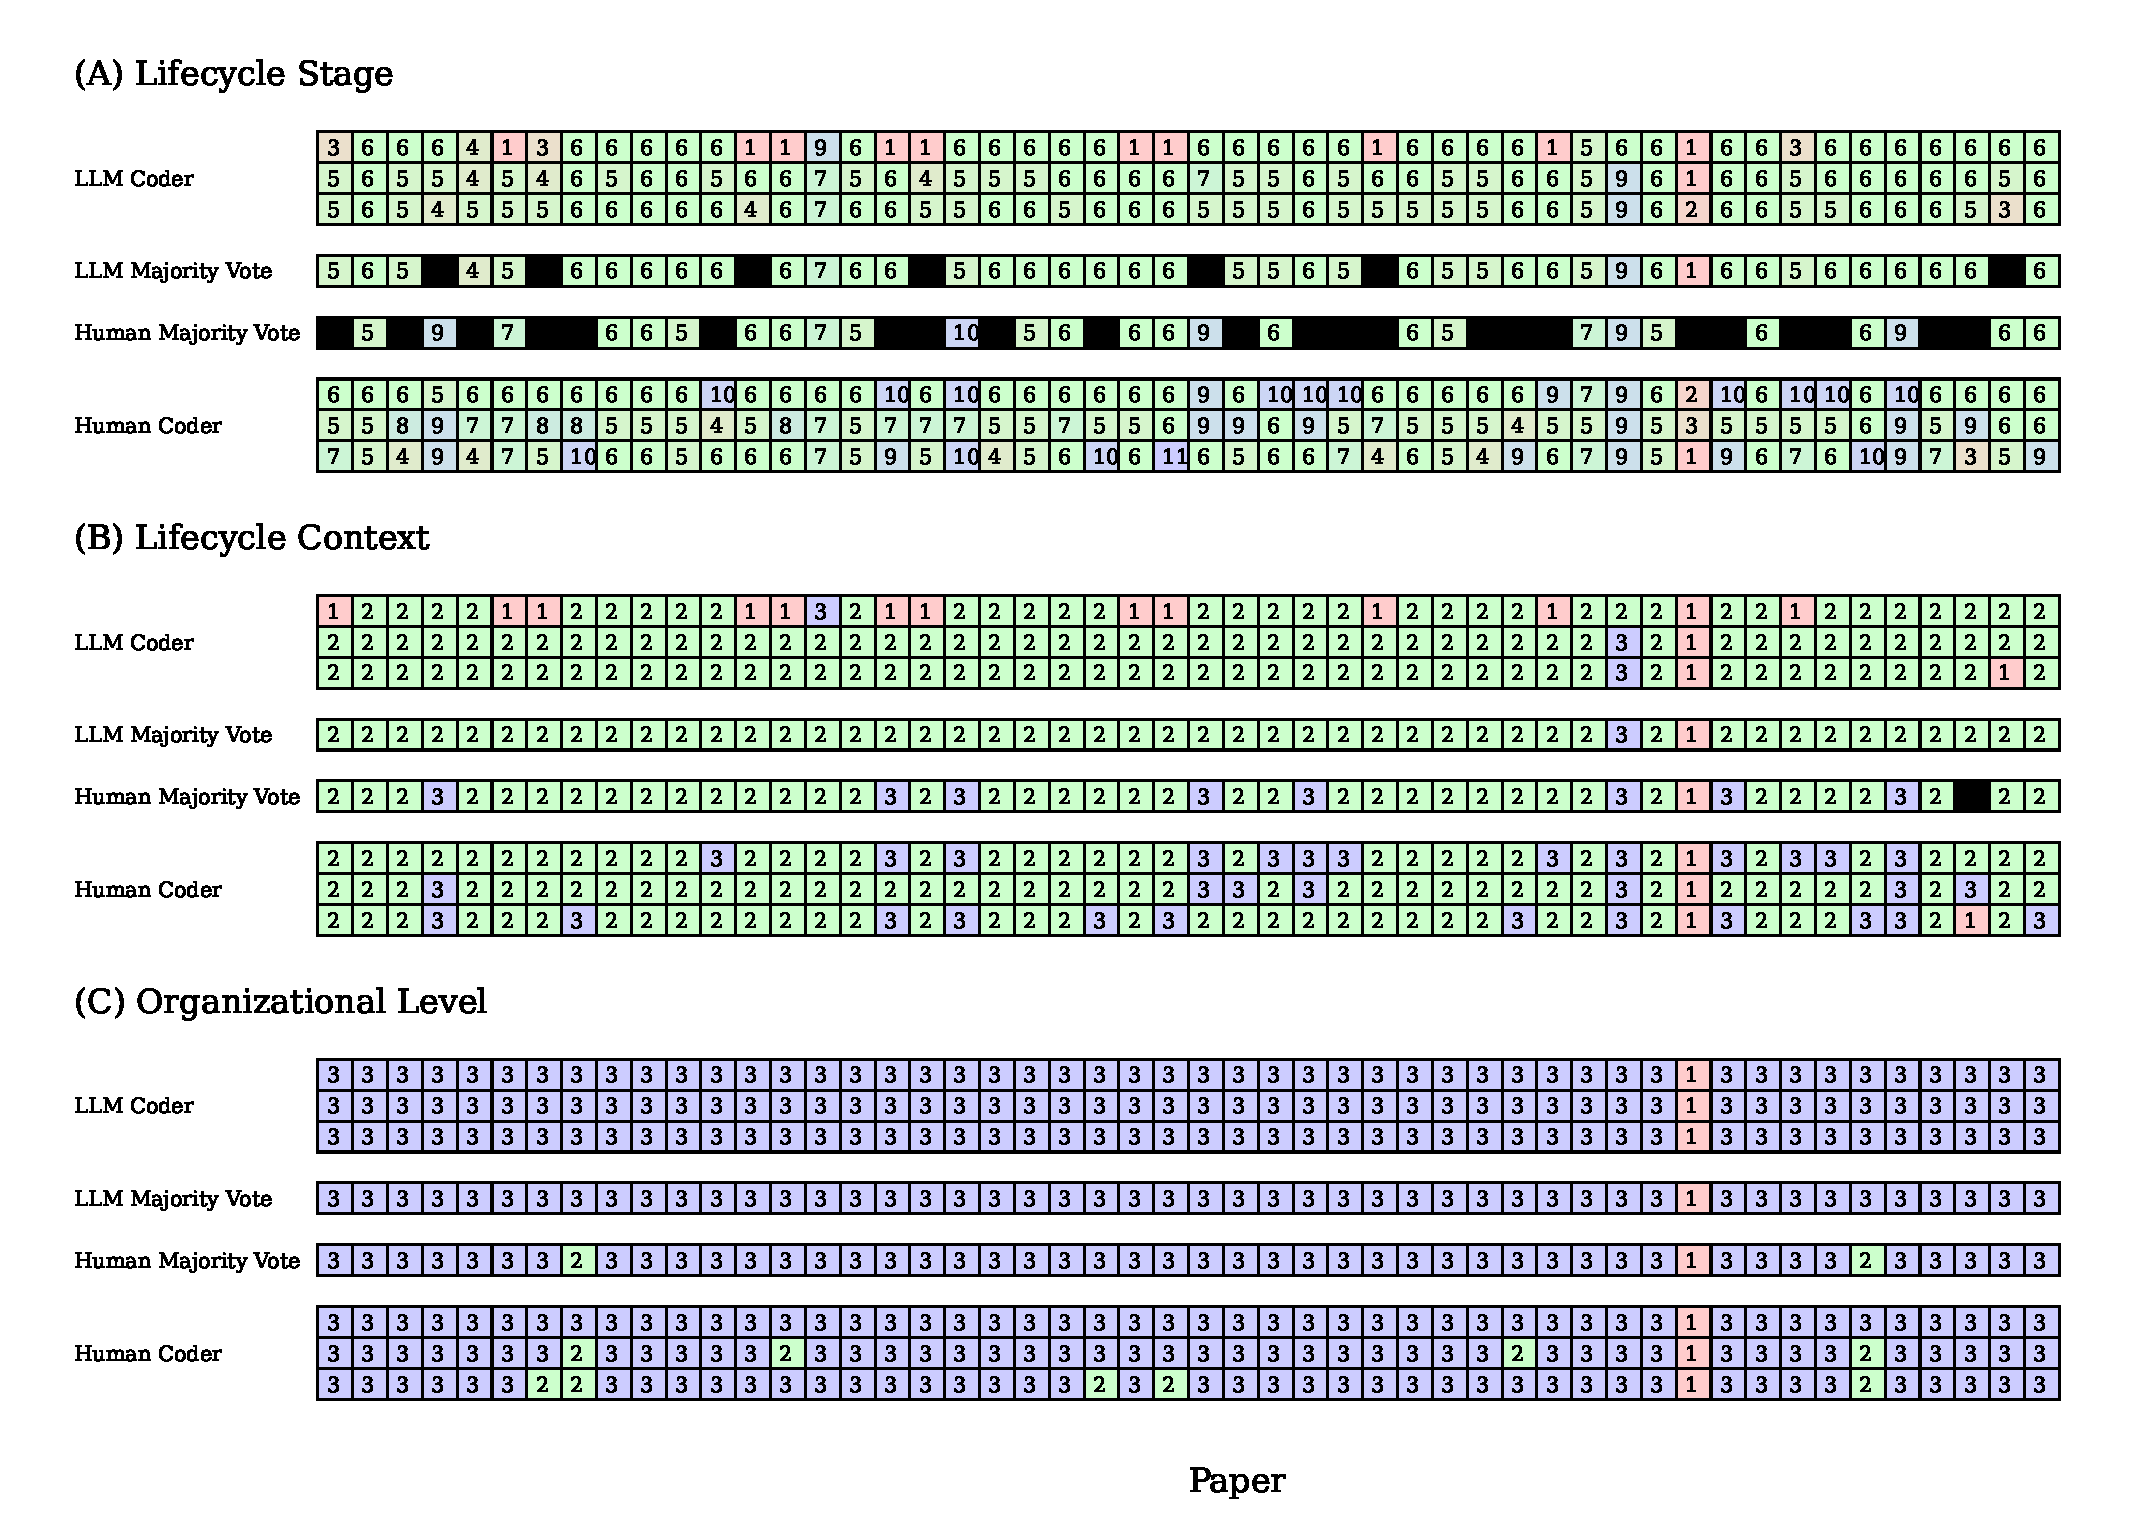
\includegraphics[width=\textwidth]{interrate.eps}
    \caption{Comparison of Human and LLM ratings on a random sample of 50 papers.  In each grid, columns correspond to papers and rows correspond to individual coders or majority votes across coder groups.  The number in each cell is the category rating (1-3 for level and context, 1-11 for systems engineering lifecycle stage, increasing from top to bottom or left to right in the categorization matrix).  Ratings are color-coded to aid visualization, with red, green, and blue corresponding to ratings 1, 2, and 3.  Individual lifecycle stages use the same color as their containing context but with a finer color gradient.  Black cells indicate papers with no clear majority vote (each coder gave a distinct rating).}
    \label{fig:interrate}
\end{figure}

\textbf{Key Takeaways:}  Our first observation is that the LLM coder group has greater internal consistency than the human coder groups, across almost all metrics and matrix axes.  This does not necessarily mean that the LLM ratings accurately reflect the paper content, but only that the LLMs have similar behavior.

Our second observation is that in almost all conditions, Krippendorff's $\alpha$ is well below 0.8, a typical threshold for reliability used in the reserch papers.  However, the IRR paper has also found that Krippendorff's $\alpha$ gives counterintuitive or paradoxical results when the rating distributions are highly skewed \cite{feinstein1990high,geijer2025some}.  This is the case in our data, since almost all papers were rated as system level (3) and solution context (2).  For example, it is clear in Figure \ref{fig:interrate}(c) that human ratings of organizational level are in high agreement, even though the corresponding Krippendorff's $\alpha$ in Table \ref{tab:inter-rataer} (bottom row, fourth column) is only 0.38.  Hence we focus on the other metrics for gauging rater reliability.

Our third observation is that ratings of systems engineering lifecycle stage are not consistent, within or across coder groups.  One explanation for this is that most papers address \textit{multiple} stages, such as system design (paper methodology), analysis (paper theoretical results), and validation (paper experimental results).  However, at the coarser resolution of lifecycle \textit{context}, there is substantially more consistency between ratings.  And organizational level ratings are highly consistent by all metrics, within and across coder groups.

Finally, and most importantly, we see that majority votes of each coder group (human and LLM) are in strong agreement, except for lifecycle stage.  This is apparent in Figure \ref{fig:interrate} and we quantify it here: For organizational level (Figure \ref{fig:interrate}(c)), the LLM majority vote matches the human majority vote in 48 of 50 papers (96\%), and for lifecycle context (Figure \ref{fig:interrate}(b)), they match in 42 of 50 papers (84\%).  This strongly suggests that, to first order, the LLM categorizations across the full $\sim 9$K paper set accurately reflect real research trends.

% We compute Krippendorff's alpha coefficients to quantify agreement between categorization approaches:

% \begin{itemize}
%     \item \textbf{Human vs. LLM Model 1}: $\alpha$ = [To be computed]
%     \item \textbf{Human vs. LLM Model 2}: $\alpha$ = [To be computed]
%     \item \textbf{Human vs. LLM Model 3}: $\alpha$ = [To be computed]
%     \item \textbf{Among Three LLMs}: $\alpha$ = [To be computed]
% \end{itemize}

% Our target threshold of $\alpha \geq 0.800$ indicates acceptable reliability for using LLM-assisted categorization while maintaining human oversight for uncertain cases.

% [Note: Actual Krippendorff's alpha values, confusion matrices, and detailed statistical analysis will be computed once all categorization results are finalized and will be inserted here.]

\begin{table}[!htbp]
\centering
\caption{Inter-Rater Reliability Metrics.}
\label{tab:interrate}
\begin{tabular}{|l|ccc|ccc|ccc|}
\toprule
Axis &  \multicolumn{3}{c}{\% Agreement} & \multicolumn{3}{c}{Krippendorff's $\alpha$} & \multicolumn{3}{c|}{Gwet's AC1} \\
\midrule
& Humans & LLMs & Both & Humans & LLMs & Both & Humans & LLMs & Both \\
Lifecycle & 0.02 & 0.30 & 0.00 & -0.02 & 0.17 & 0.07 & 0.12 & 0.44 & 0.27 \\
Context & 0.60 & 0.70 & 0.36 & 0.28 & 0.12 & 0.15 & 0.66 & 0.77 & 0.68 \\
Level & 0.86 & 1.00 & 0.86 & 0.38 & 1.00 & 0.43 & 0.90 & 1.00 & 0.94 \\
% Fine & 0.02 & 0.30 & 0.00 & -0.01 & 0.18 & 0.07 & 0.14 & 0.44 & 0.29 \\
% Coarse & 0.56 & 0.70 & 0.36 & 0.27 & 0.13 & 0.15 & 0.65 & 0.78 & 0.68 \\

\bottomrule
\end{tabular}\label{tab:inter-rataer}
\end{table}
\chapter{Gaps and Recommendations}
\section{Gaps}

%\noindent\fbox{\parbox{\dimexpr\textwidth-2\fboxsep-2\fboxrule}{%
%\begin{center}
\begin{tcolorbox}
\textbf{AI trustworthiness research is overwhelmingly focused on the technical solutions context, with major gaps in the problem or mission and trustworthiness contexts.}
\end{tcolorbox}
%\end{center}
%}}\\
%\newline

When we step back and look at the paper publications as a whole, a clear problem emerges. The effort to build ``trustworthy AI'' is overwhelmingly focused on technical solutions, while largely ignoring the mission and governance context those systems are supposed to serve. When we mapped the papers to the NIST SP 800-39 organizational tiers and the ISO/IEC/IEEE 15288 lifecycle, over 95\% of the work landed at the technical System Level (Row 3) and 83\% in design and integration of components within the solutions space. In other words, we are building systems before we have clearly defined what they are being built for. \newline

\begin{figure}[h]
    \centering
    \includegraphics[width=\textwidth]{STORM-AI Deliverable-1/Figures/CoreSummary.png}
    \caption{Data displayed in percentages based on context categories}
    \label{fig:llm3_scoring_percentage}
\end{figure}

Across the paper publications, a consistent pattern emerges. The body of work forms a distinctly bottom-heavy pyramid, with more than 83\% of research concentrated at the technical System Level and less than 15\% addressing organizational governance. In defense and other high-consequence domains, this imbalance is problematic. Technical sophistication cannot compensate for weak governance structures or poorly defined mission requirements.

This skew also reflects a broader tendency toward solution-first thinking. The heavy emphasis on System Analysis and Design Definition suggests the field is producing tools, algorithms, and architectures faster than it is defining the problems they are meant to solve. Business analysis, stakeholder needs, and requirements definition—where purpose, constraints, and success criteria should be established—receive comparatively little attention.

As a result, foundational work is often missing altogether. Core questions remain unanswered: what mission outcomes justify trust, what stakeholders actually require from AI-enabled systems, and how organizational policy should shape AI adoption. These are not peripheral concerns; they are prerequisites. Without answering them, technical solutions are designed in a vacuum.

The consequences are visible downstream. Verification and validation are sparsely represented in the published papers, with only 802 papers addressing verification and 276 addressing validation. This signals a lack of emphasis on demonstrating that AI systems actually meet their stated trustworthiness objectives in real operational settings. In defense contexts, where failure can have severe and irreversible consequences, this gap is especially concerning.

Finally, the transition from development to operations is largely neglected. With only 61 papers on transition, there is little guidance on how reliable AI systems should be securely deployed, integrated, and handed over to operational users. However, this phase is where trust is most likely to erode if governance, controls, and accountability are not firmly in place.

This imbalance becomes more concerning as you move up the stack. Only 1\% of the work addresses the Organizational Level (Tier 1), and just 3\% addresses the Mission or Business Process Level (Tier 2). Even more striking is the lack of attention paid to the early stages of the lifecycle, phases—Business and Mission Analysis and Stakeholder Needs and Requirements Definition. These are the phases in which the purpose, the constraints, and the success criteria are supposed to be defined. Yet, they receive less than 3\% attention in the research efforts.

This is not just a philosophical issue; it directly contradicts established systems security engineering guidance. NIST SP 800-160 is clear that trustworthiness starts with stakeholder needs and protection requirements and must be carried through the entire life cycle. If mission intent and requirements are poorly defined—or missing altogether—there is no way to compensate for that later. Cyber resiliency, mission assurance, and security analysis all depend on having a well-defined operational context from the start.

This problem is amplified by the current AI deployment landscape. The State of AI in Business 2025 report shows that despite heavy investment and widespread adoption, roughly 95\% of custom enterprise AI solutions fail to reach production. The reasons are familiar: brittle workflows, lack of context, and poor alignment with real operational needs. \cite{ChallapallyEtAl2025StateOfAI} AI is increasingly being built as a general-purpose tool rather than as a mission-specific system. As a result, these systems lack the persistence, memory, and adaptability required for high-stakes environments, and users default back to human judgment when complexity increases.

Addressing this requires a shift in priorities. If we want AI systems that are genuinely trustworthy, we must start by doing the hard early work: explicit mission elicitation, clear organizational risk framing, and well-defined stakeholder requirements at Tiers 1 and 2. This is how we move from building clever solutions to solving the right problems. Only then can security and trustworthiness be demonstrated, rather than assumed.

\section{Preliminary Recommendations}

Addressing the documented gap in early-lifecycle mission context and requirements demands a disciplined, systems-level approach. We therefore recommend applying the System-Theoretic and Technical Operational Risk Management (STORM) methodology \cite{STORM}, with particular emphasis on its STPA-SEC component \cite{STPA-SEC}. STPA-SEC is explicitly designed to do the work that is currently missing: eliciting mission objectives, identifying unacceptable losses and hazards, and defining the constraints that must govern system behavior. In doing so, it aligns policy intent with technical implementation and frames security as a mission problem rather than a purely technical one. 

%\noindent\fbox{\parbox{\dimexpr\textwidth-2\fboxsep-2\fboxrule}{%
%\begin{center}
\begin{tcolorbox}
\textbf{There is a clear opportunity to strengthen mission context, early requirements definition, and downstream verification and validation in AI trustworthiness research.}
\end{tcolorbox}
%\end{center}
%}}
%\newline

Once these mission requirements and constraints are established, STORM's Certified Security by Design (CSBD) component \cite{CSBD-IOT} \cite{CSBD-Education} enables formal verification that the system design satisfies them. CSBD provides evidence---not assumptions---that the implemented Concepts of Operation (CONOPS) enforce complete mediation, ensuring that actions occur if and only if they are authorized and authenticated under the defined policy. This closes the loop between mission intent, system design, and verification, and delivers the kind of demonstrable trustworthiness and mission assurance required by NIST SP 800-160v1r1 \cite{nist_sp800_160v1}.

%% ---------------------------------------------------
%% Works Cited
%% ---------------------------------------------------
%\chapter{Works cited}
%\label{ch:works-cited}

%\begin{enumerate}
%\item National Cyber Security Centre et al. \textit{Guidelines for secure AI system development}. 2023. \\
%\url{https://www.ncsc.gov.uk/files/Guidelines-for-secure-AI-system-development.pdf}
%\item 
%\end{enumerate}

%% ---------------------------------------------------
%% Bibliography from BibTeX
%% ---------------------------------------------------
%\typeout{}
%\bibliographystyle{acm}
\bibliographystyle{plainnat}
\bibliography{Book,references,chapter6_references}
% \printbibliography
% \addcontentsline{toc}{chapter}{Bibliography}

\end{document}
